\chapter{Time-Series Representations}
\label{cha:representation}
As mentioned in Chapter~\ref{ch:background}, in many time-series classification tasks, a simple KNN with well-extracted features is able to produce a competitive results with other more sophisticated models. In recent years, various novel time-series representation algorithms are proposed, most of them outperform the previous baseline in the context of classification tasks. However, \textbf{there are rare studies about the effectiveness of them in the time-series clustering tasks}. By research, we find that some representation methods can achieve certain invariances, and we try to apply them to stock clustering to test their effectiveness.\\
\\Generally, time-series data representations can be categorized into three groups. As seen in Figure~\ref{fig:representation1}, there are three major ways to fed the preprocessed data into clustering models. The left group of approaches are mainly statistics-based, they generally require two steps: (1) extracting static features from the original sequences either globally or locally. Here ``globally'' means using the information of a whole sequence to form a feature vector, while ``locally'' requires segmenting the whole sequence into subsequences first, extracting the features individually and then concatenating the features to form a feature vector; (2) selecting features, filtering out features that may decrease the perfomance of clustering algorithms and reserving the most discriminative features. The right group of approaches represent clustering algorithms that directly take the processed time-series data as input, their perfomance is highly associated with the similarity measure. The middel block represents various representation schemes that try to project the original sequences into discriminative feature space, extract the hidden structure of the data. In this chapter, we mainly introduce some traditional and novel algorithms of the left and the middel blocks.
\begin{figure}[!htbp]
    \centering
    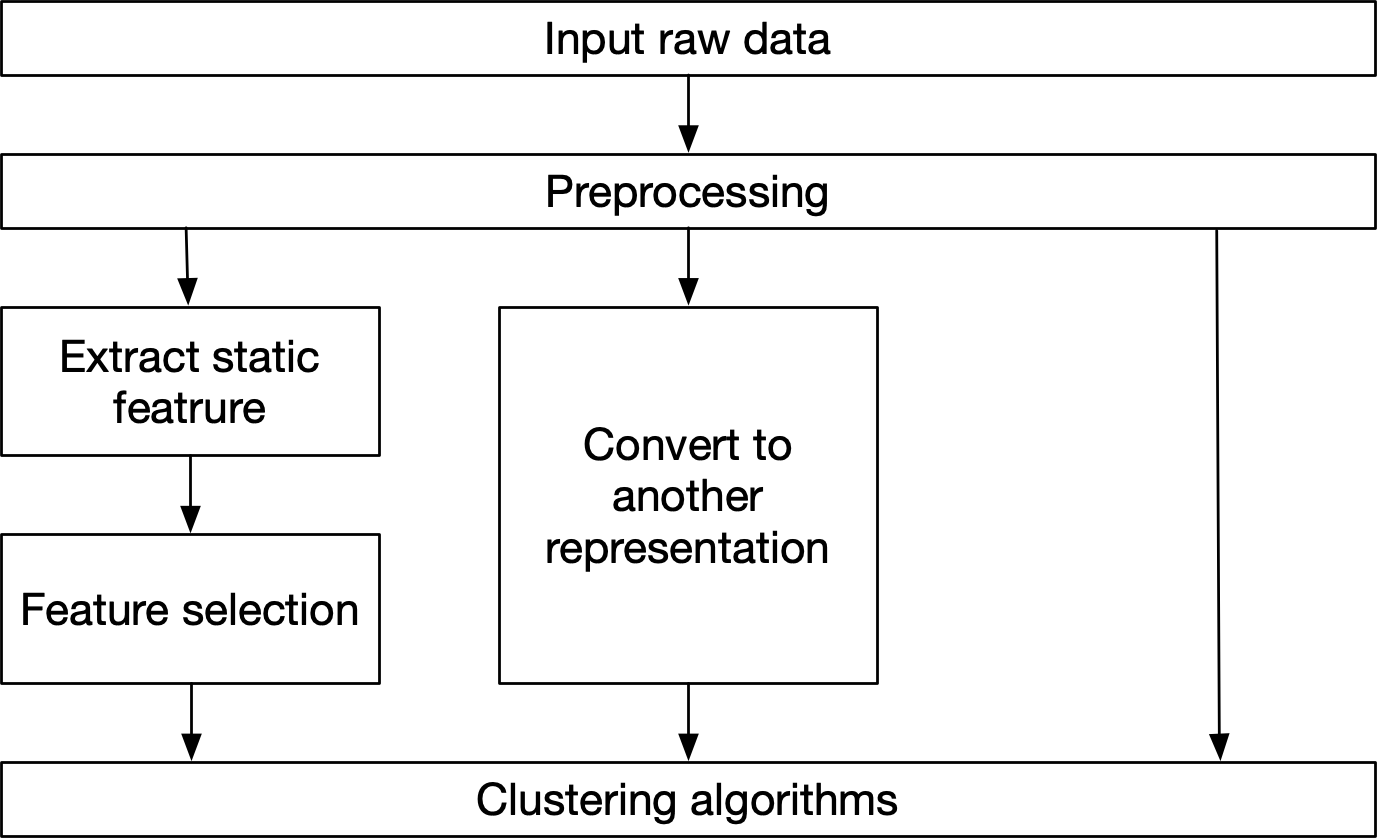
\includegraphics[width=0.5\columnwidth]{representation1.png}
    \caption{Approaches for time-series data clustering}
    \label{fig:representation1}
\end{figure} 

\section{Static Feature Representation}

\subsection{Statistical features representations}
\textbf{Statistical features} are the most common and well-known features of time-series data. Compared with raw data, those statistics features are less sensitive to noise and distortion. Compared with other representations, this representation is easy to obtain. Due to these two attributes, statistical features representation is regarded as the baseline of time-series representation problems. \cite{nanopoulos2001feature} firstly examine this representation in time-series classification tasks, then, such representation is applied to clustering tasks. \\
\\According to \cite{nanopoulos2001feature}, statistical features can be divided into two groups: (1) first-order features, which can be computed directly from the actual value of data; (2) second-order features, which are computed from the difference of nearby values. For time-series data, the second-order features are computed from a transformed time series $y_t\prime = y_{t+D} - y_t$ ($1 \le t \leq n-D$), where $D$ is a user-defined gap between the points in the time series being compare. Some common statistical features include: (1) the mean value $\mu$; (2) the standard deviation $\sigma$; (3) the skewness $SKEW$; (4) the kurtosis $KURT$. The latter two features indicate the shape of the sequence's value distribution. Skewness representation the magnitude of asymmetry (a sequence is symmetric if it looks the same to the left and right of the center point). Kurtosis indicates the degree of peakedness of a distribution relative to a normal distribution (a distortion is flat if it has more outliers). Their equation are:
\begin{equation} 
    \mu = \frac{\sum_{t=1}^n y_t}{n} \\
\end{equation}
\begin{equation} 
    \sigma = \sqrt{\frac{\sum_{t=1}^n (y_t - \mu)^2}{n}}
\end{equation}
\begin{equation}
    SKEW = \frac{\sum_{t=1}^n (y_t-\mu)^3}{n\sigma^3}
\end{equation}
\begin{equation} 
    KURT = \frac{\sum_{t=1}^n (y_t-\mu)^4}{n\sigma^4} - 3
\end{equation}
Extracting the four features from $y_t$ and $y_t\prime$ forms the first-order and second-order representation respectively. The first-order features solely can represent the original data, but it can also be concatenated with the second-order features to form a better representation. Figure~\ref{fig:nycbelp1} shows an example of this representation transformation. The samples used here are the records of stock ``NCYB'' and ``ELP'' in 2011. Both first and second order features are used, and the gap $D$ is set to 5. Note that the features include the mean and standard deviation, and hence the samples here are not normalised.
\begin{figure}[!htbp]
    \centering 
    \subfigure[Original sequences] { \label{fig:nycbelpsub1} 
    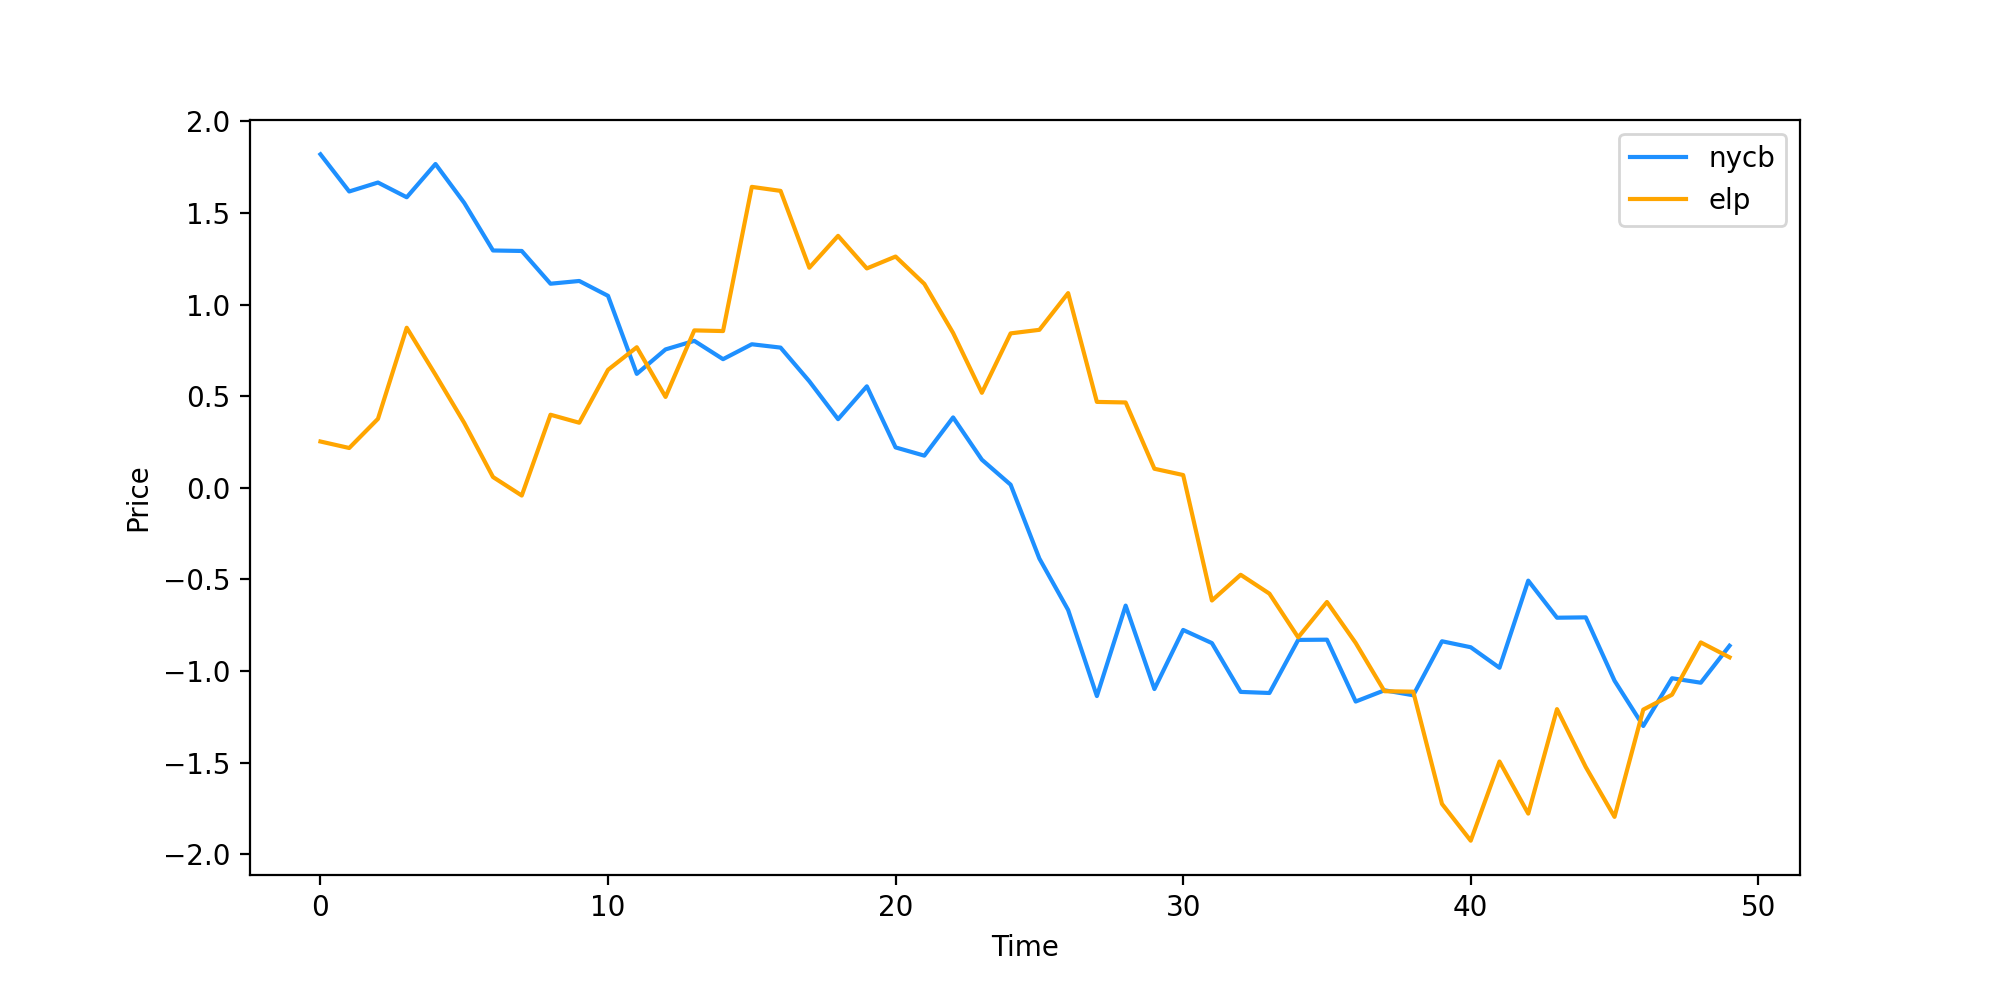
\includegraphics[width=0.4\columnwidth]{nycbelp1.png} 
    } 
    \subfigure[Statistical features representation] { \label{fig:nycbelpsub2} 
    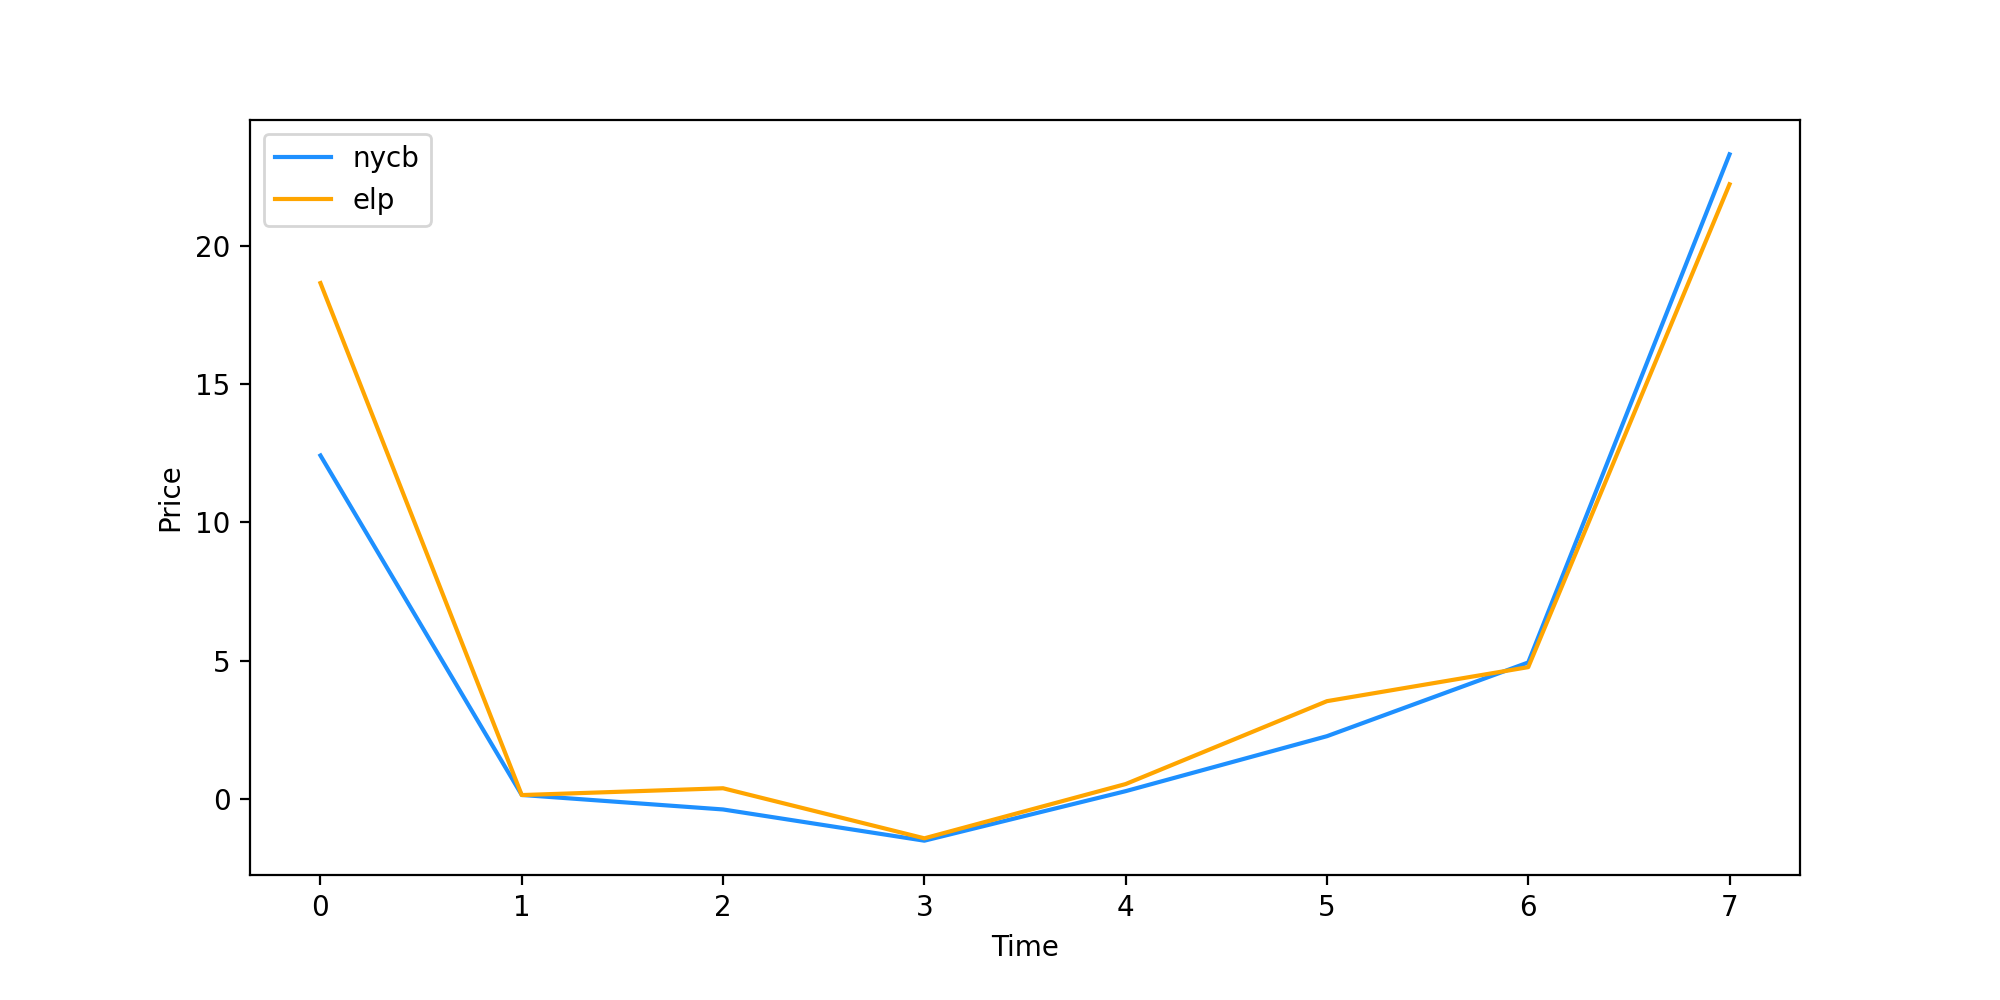
\includegraphics[width=0.4\columnwidth]{nycbelp2.png} 
    } 
    \caption{Example of statistical features representation} 
    \label{fig:nycbelp1} 
\end{figure} 

\subsection{Bag-of-patterns representation}
Bag-of-words (BOW) is one typical and traditional static feature representation method. It was wildly used in natural languages processing and image processing until more powerful representation learning algorithms came out. Similarly, time-series sequences can be represented by pattern histograms, and such representation is call \textbf{Bag-of-Patterns} \cite{lin2012rotation}.\\
\\Generally, BOW requires computing a $p$-by-$q$ martrix $X$. In the context of document representation, $p$ denotes the the number of unique terms in the whole corpus, $q$ is the number of documents, and the element $X_{i,j}$ represents the frequency of the word $i$ occurring in the document $j$. Document $j$ then can be represented by the $j$th column of $X$. In the context of time-series representation, \cite{lin2012rotation} define $p$ as the number of unique SAX strings and $q$ as the number of sequences. Different from sentences, sequences are consecutive and have no ``delimiters'', therefore, there is no obvious definition of ``words''. To solve this problem, \cite{lin2012rotation} use sliding window to separate the original sequence into subsequences, and apply Symbolic Aggregate approXimation (SAX) to each frame. The intuition of using SAX here is that SAX is a symbolic representation for time-series and can convert each frame into a SAX word (a string), which follows the definition of BOW. The details of SAX are described in \cite{lin2007experiencing}. To be brief, SAX is developed on the PAA representation discussed before, it takes two parameters from users: (1) $\alpha$: the size of the alphabet to use; (2) $w$: the size of the words to produce. Similar to PAA, it first splits the original sequences into $w$ frames, and calculate the mean value within each frame. Each mean value (or called coefficient) is then mapped to specific a symbol based on a distribution that are divided into $\alpha$ equiprobable regions. Note that when the sequences are normalised, the distribution is more likely to be a Gaussian. Figure~\ref{fig:sax1} shows an example of SAX transformation with $\alpha$ set to 5. \\
\begin{figure}[!htbp]
    \centering
    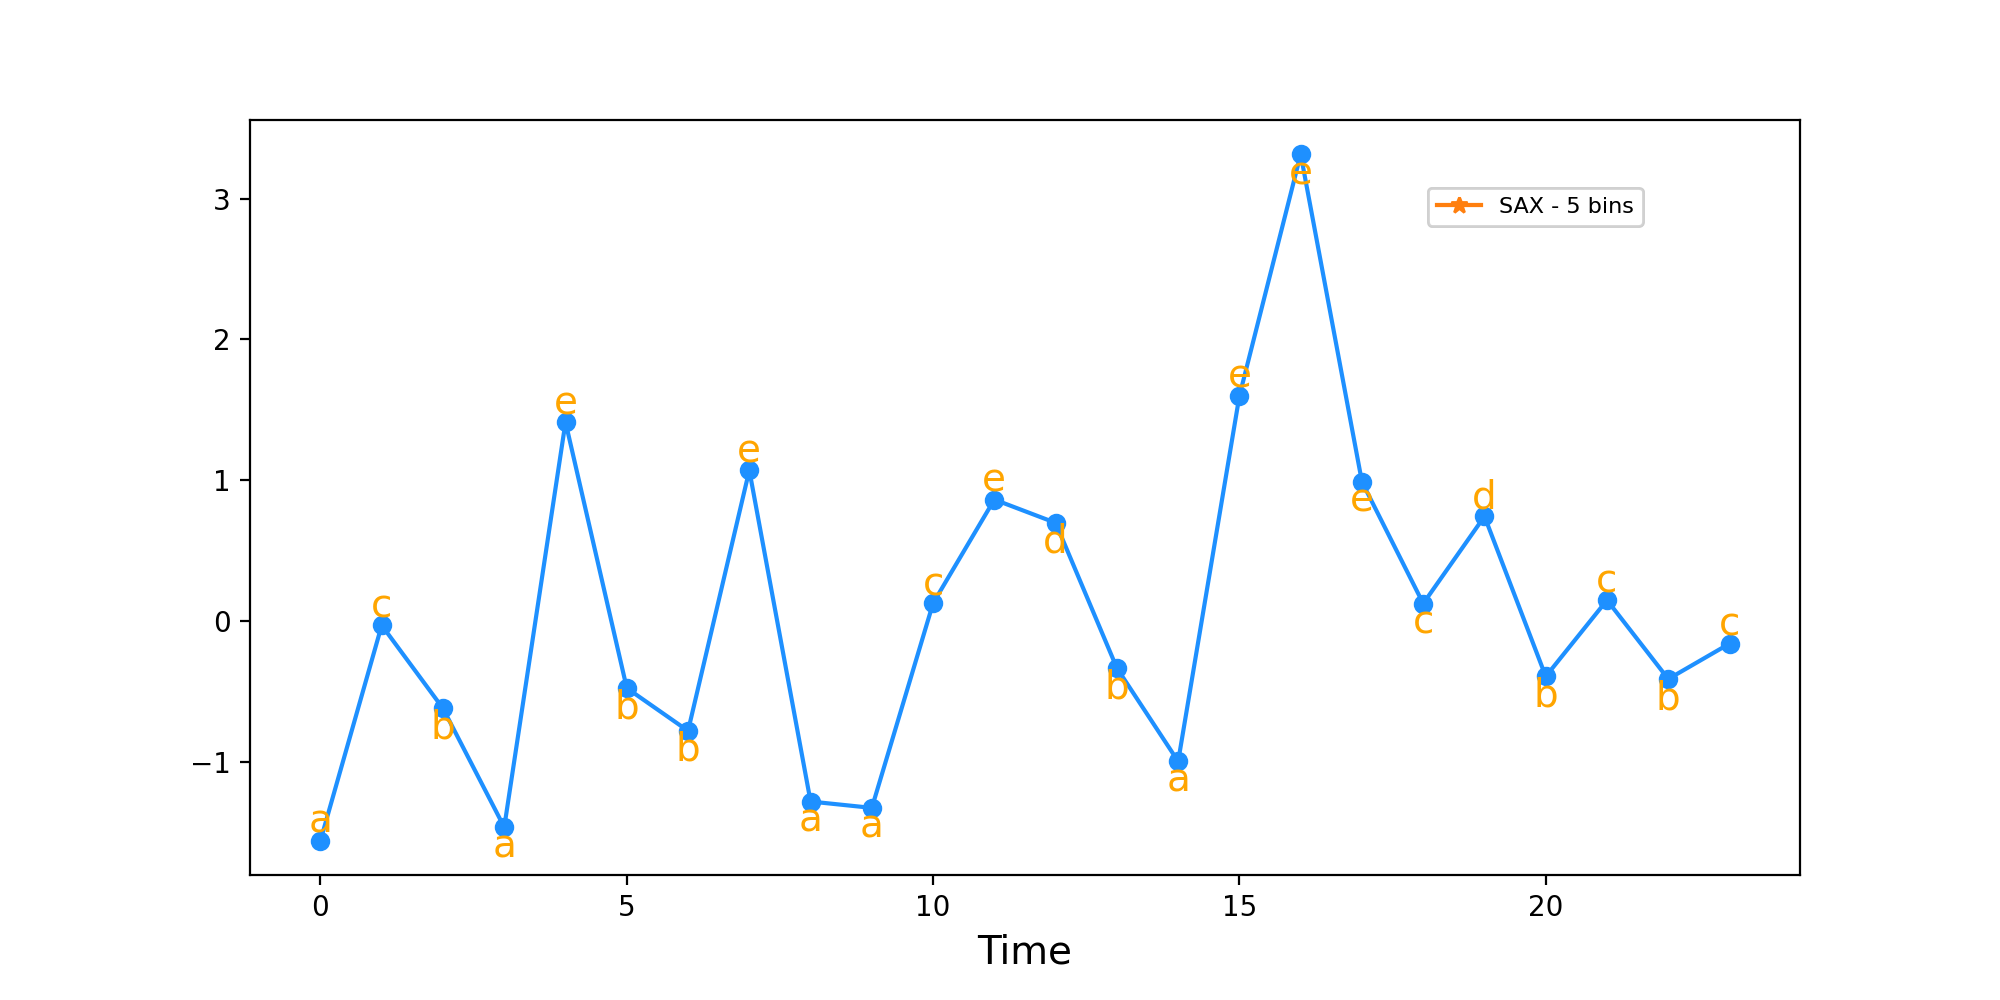
\includegraphics[width=0.6\columnwidth]{sax1.png}
    \caption{Example of SAX transformation}
    \label{fig:sax1}
\end{figure} 
\\After the transformation, each frame is assigned with a string, and the ``term-document'' martrix can be constructed. It should be noted that in some regions (especially smooth regions), neighbouring subsequences could be assigned with the same string, and this may result in over-counting issue. One feasible way to solving the problem is called Numerosity Reduction, which merely records the starting point of a set of consecutive subsequences that are mapped with the same string. One example of Numerosity Reduction provided by \cite{lin2007experiencing} is that, given a SAX transformed sequence S as follows:
\begin{equation}\nonumber
    S = aac~acc~abc~abb~abb~abb~abb~bac~baa
\end{equation}
Its reduced form is defined as:
\begin{equation}\nonumber
    S\prime = aac_1~abc_3~abb_4~bac_8~baa_9
\end{equation}
As stated by \cite{lin2012rotation}, the effect of this issue highly depends on the data. In terms of sequences that a generally smooth, dealing with the over-counting problem is required. For other sequences, that may not necessary. Figure~\ref{fig:bop1} shows an toy example of Bag-of-Patterns transformation, for better comparison, the result is expressed in a bar chart. The samples used here are the processed sequences of ``IBA'' and ``WPZ'' in 2011. Their BOP representations are quite different, which is comply with their real trend. 
\begin{figure}[!htbp]
    \centering 
    \subfigure[Original sequences] { \label{fig:sample2} 
    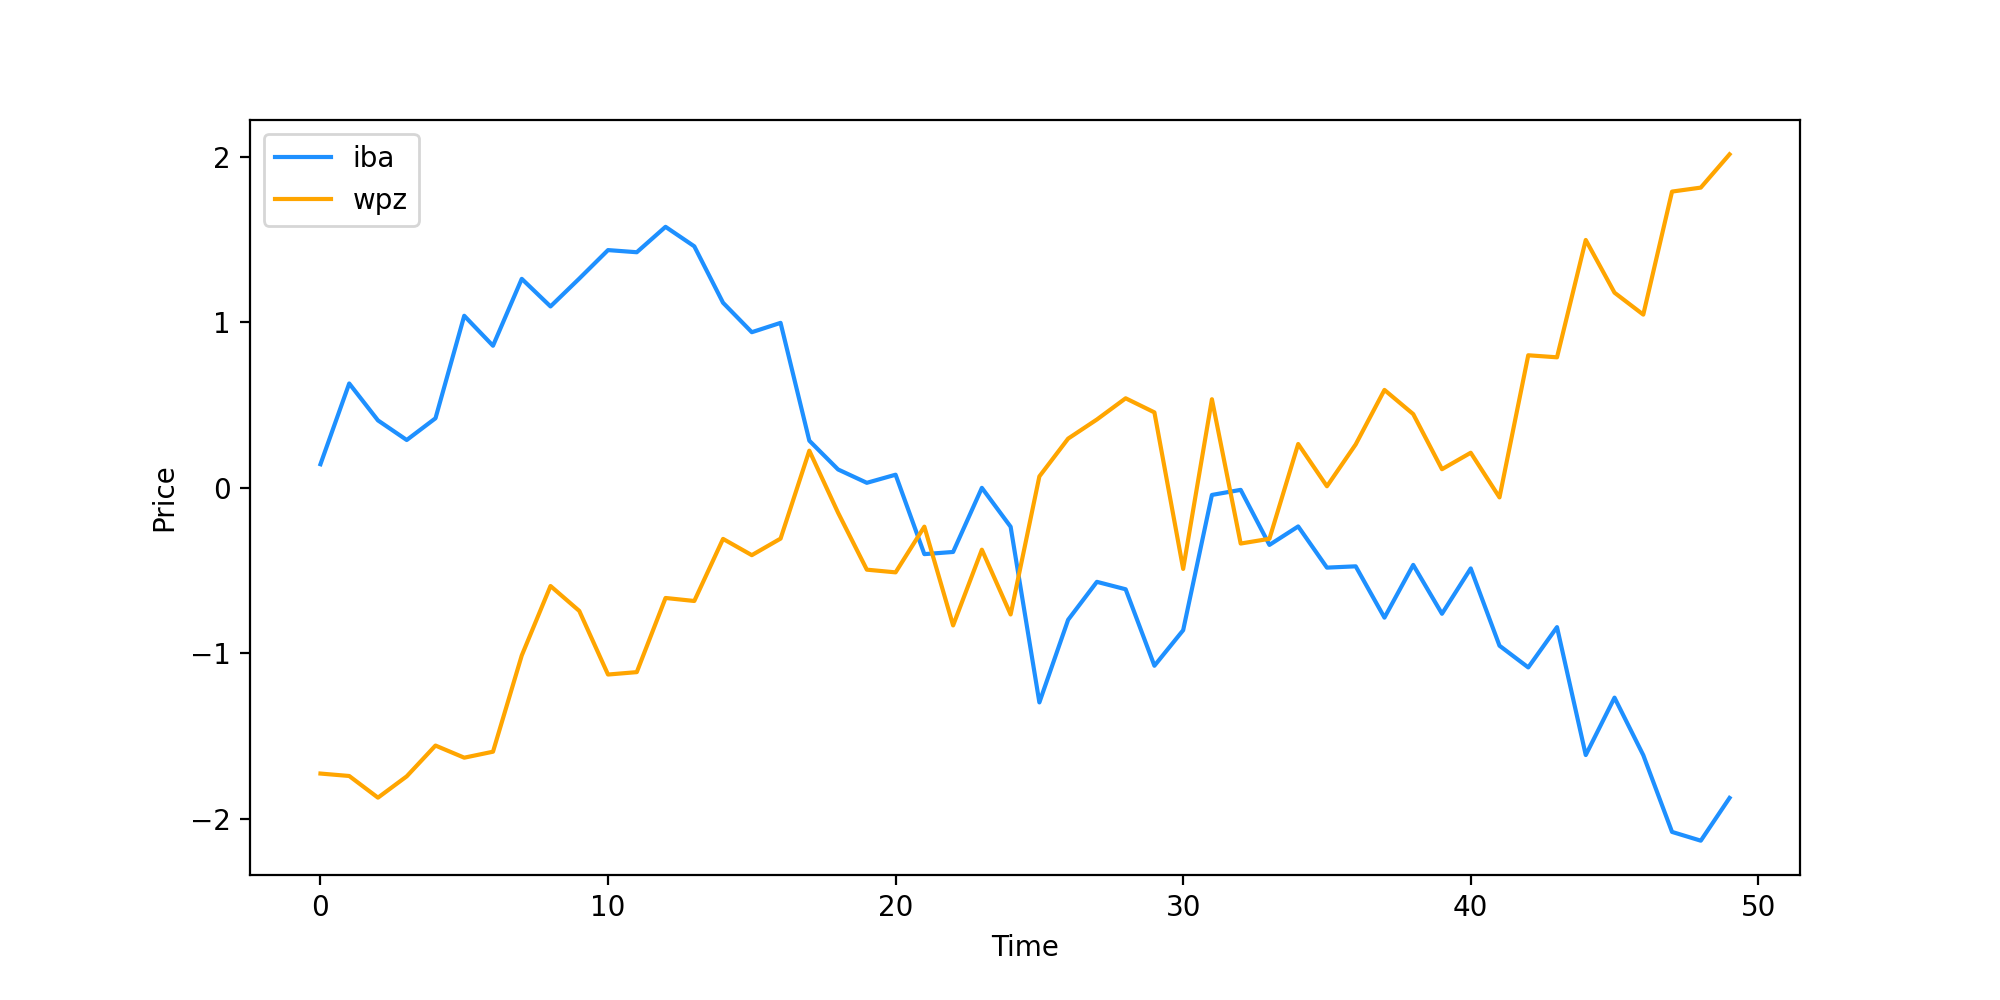
\includegraphics[width=0.4\columnwidth]{ibawpz.png} 
    } 
    \subfigure[BOP representation] { \label{fig:bopsub1} 
    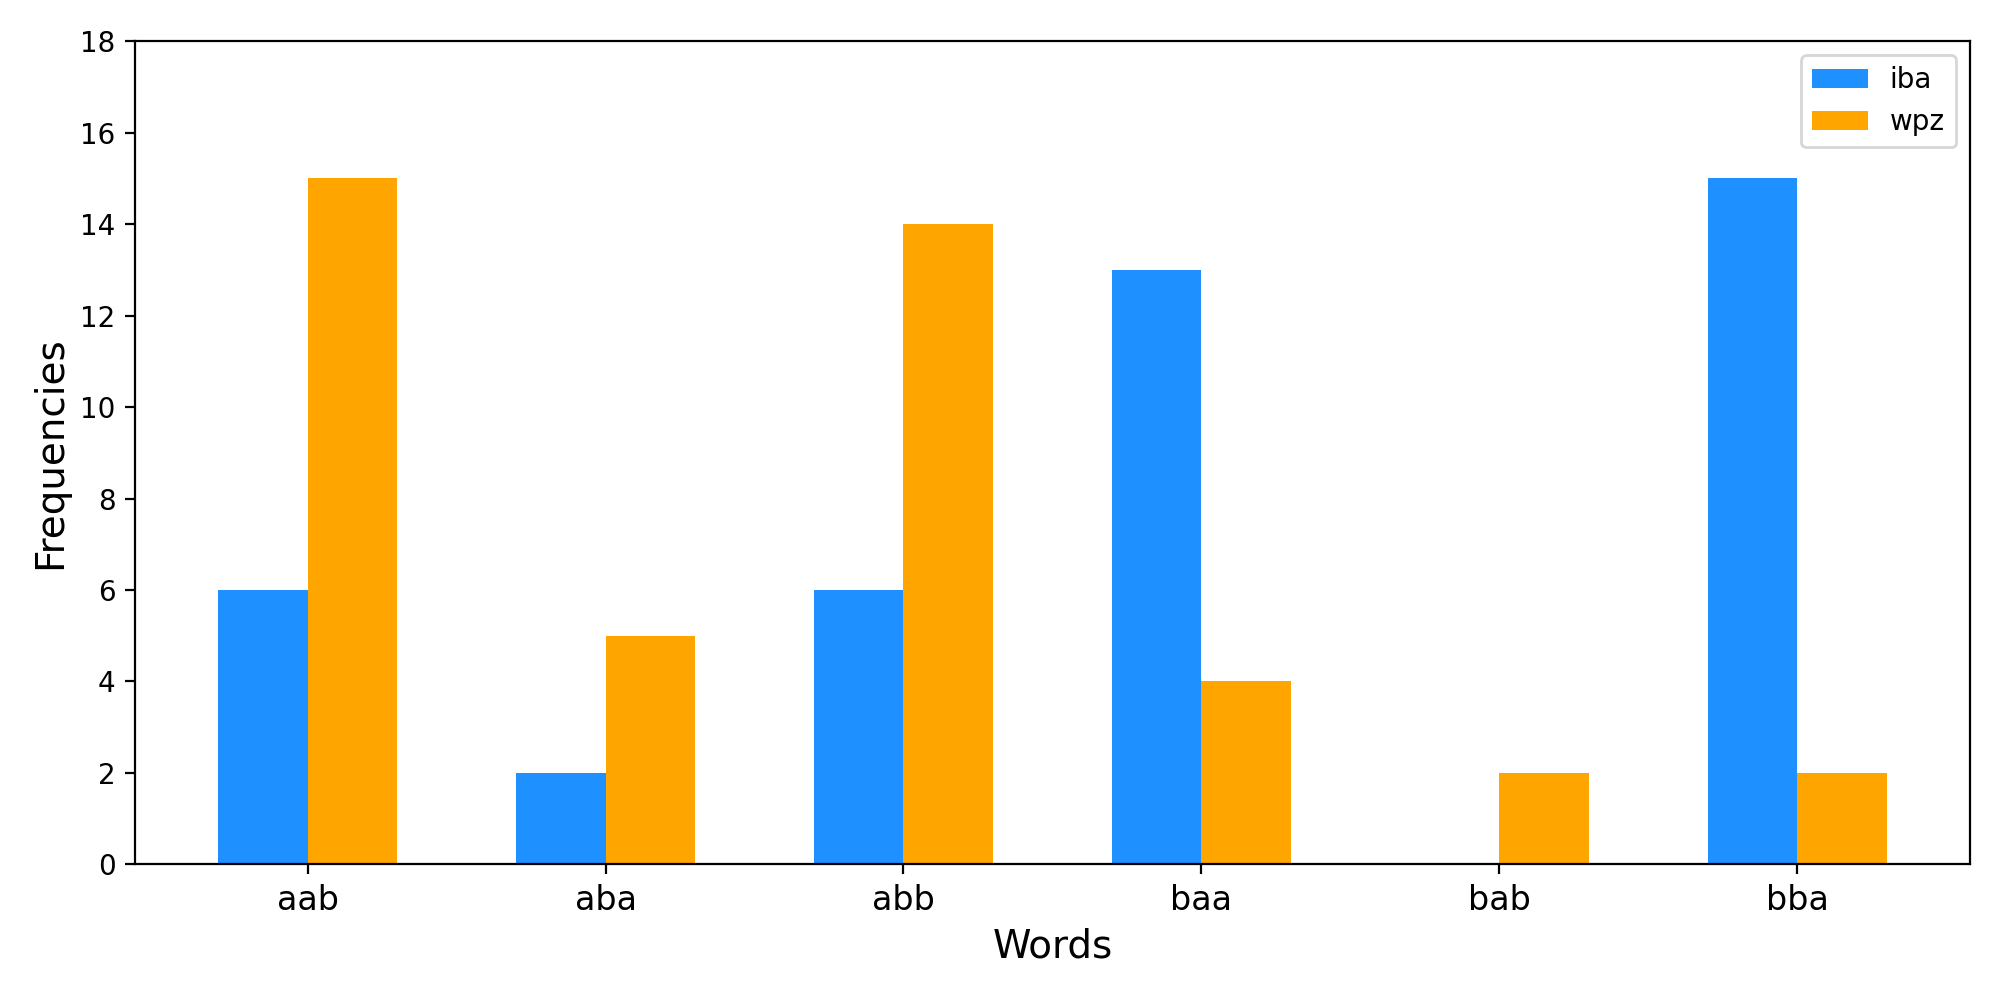
\includegraphics[width=0.4\columnwidth]{bop1.png} 
    } 
    \caption{Example of Bag-of-Patterns representation} 
    \label{fig:bop1} 
\end{figure} 

\subsection{Path signature representation}
\textbf{Path signature} \cite{chen1958integration} is a relatively novel representation method for non-smooth paths, it is the core part in rough path theory. The term ``rough path'' denotes a sequence that is continuous but highly oscillatory and therefore has no derivatives of all orders. One typical example is a stock price stream, which can be regarded as a result of Brownian movement. In the rough path theory, each rough path can be decomposed into a set of infinite path integrals, and that set is called the signature of the path. A brief mathematical definition could be: given a sequence (continuous or discrete) $P = (P_1, P_2, \cdots, P_T) \in \mathbb{R}^{T \times D}$, where T is number of points in the sequence, D is the dimension of each data point, let $P_t^i$ denotes the i-th attribute of point $P_t$ $(1\le t\le T, 1 \le i \le D)$, the whole sequence can be represented by n-fold iterated integral over the sequence (n could be infinite). The simplest case is that when $D = 1$, the 1-fold representation of P is a real value defined as:
\begin{equation}
    S(P)_{1,T}^1 = \int_{1 < t \le T}dP_t^1 = P_T^1 - P_1^1
\end{equation}
Similarly, the 2-fold representation is also a real value:
\begin{equation}
    S(P)_{1,T}^{11} = \int_{1 < t \le T} S(P)_{1,T}^1dP_t^1 = \frac{1}{2} (P_T^1 - P_1^1)^2
\end{equation}
The k-fold representation is: 
\begin{equation}
    S(P)_{1,T}^{11\cdots 1} = \frac{1}{k!} (P_T^1 - P_1^1)^k
\end{equation}
The final signature representation of sequence P is the vector $(S(P)_{1,T}^1, S(P)_{1,T}^{11}S(P)_{1,T}^{11\cdots 1}) \in \mathbb{R}^k $ , whose dimension k is the number of fold wanted by users.\\
When D = 2, 1‐fold representation has 2 elements defined as follows:
\begin{equation}
    \begin{aligned}
        S(P)_{1,T}^1 = \int_{1 < t \le T}dP_t^1 = P_T^1 - P_1^1 \\
        S(P)_{1,T}^2 = \int_{1 < t \le T}dP_t^1 = P_T^2 - P_1^2
    \end{aligned}
\end{equation}
2-fold representation has $D^2 = 4$ elements:
\begin{equation}
    \begin{aligned}
        S(P)_{1,T}^{11} & = \int_{1 < t \le T} S(P)_{1,T}^1dP_t^1 = \frac{1}{2} (P_T^1 - P_1^1)^2 \\
        S(P)_{1,T}^{22} & = \int_{1 < t \le T} S(P)_{1,T}^1dP_t^1 = \frac{1}{2} (P_T^2 - P_1^2)^2 \\
        S(P)_{1,T}^{12} & = \int_{1 < t_1 \le T}\int_{1 < t_2 \le T}dP_{t_1}dP_{t_2} \\
        S(P)_{1,T}^{21} & = \int_{1 < t_2 \le T}\int_{1 < t_1 \le T}dP_{t_2}dP_{t_1}
    \end{aligned}
\end{equation}
In general, when D = d, the i-th element of k-fold representation can be seen in eqaution \ref{func:sig1}, where $(n_1,n_2, \cdots, n_k) \in \{1, \cdots, k\}$:
\begin{equation}
    \label{func:sig1}
    S(P)_{1,T}^{n_1,n_2,\cdots, n_k} = \int_{1 < t_k \le T} \cdots \int_{1 < t_3 \le t_4} \int_{1 < t_2 \le t_3}dP_{t_1}^{n_1}dP_{t_2}^{n_2} \cdots dP_{t_k}^{n_k}
\end{equation}
The final signature of the whole path P is the collection of all elements in every fold defined as follows:
\begin{equation}
    \begin{aligned}
        S(P)_{1,T} = (& 1, S(P)_{1,T}^1, \cdots, S(P)_{1,T}^D), \\
        & S(P)_{1,T}^{1,1}, \cdots, S(P)_{1,T}^{2,1}, \cdots, S(P)_{1,T}^{D,1}, \cdots, S(P)_{1,T}^{D,D}, \\
        & S(P)_{1,T}^{1, 1,\cdots, 1}, \cdots, S(P)_{1,T}^{n_1, n_2,\cdots, n_k}, \cdots, S(P)_{1,T}^{D,D,\cdots,D}, \cdots)
    \end{aligned}
\end{equation}
Conventionally, the first term is set to 1. With the increment of fold k, the collection could be infinite. However, in practice, there is no need of using a large k, users can decide the k based the the dimension formula of the final vector: $\omega(D,k) = (D^{k+1} - 1) (D-1)^{-1} $. The truncated elements are regarded as the path signature feature of the original sequence, and then can be used in further analysis. A promising property of path signature representation is that each term of it has a physical meaning and can reveal the shape information of the path. For example, the first order terms $S(P)_{1,T}^i = P_T^i-P_1^i$ ($i=1,\cdots,k$) denotes the increments of the path. Higher order terms can be interperted as generalised polynomials of paths \cite{chevyrev2016primer}.\\
\\It's worth noting that path signature should be applied to multi-variable sequences since from the eqaution, higher order term $S(P)_{1,T}^{1_1,\cdots,1_k} = \frac{1}{k!}(P_T^1-P_1^1)^k$ is merely an function of the increment $P_T^1-P_1^1$. To apply this representation method to univariate sequences, one feasible way is adding at least one new feature. This new feature could be the time axis, or the features generated by lead-leg transformation. The equations below show the process of lead-leg transformation. As stated by \cite{chevyrev2016primer}, such transformation makes path signature able to capture the quadratic variation of sequences, which is crucial in finacial applications. 
\begin{equation}
    P_j^{lead}=
    \begin{cases}
    P_{t_i}& \text{if j=2i}\\
    P_{t_i}& \text{if j=2i-1}
    \end{cases}   
\end{equation}
\begin{equation}
    P_j^{lag}=
    \begin{cases}
    P_{t_i}& \text{if j=2i}\\
    P_{t_i}& \text{if j=2i+1}
    \end{cases}   
\end{equation}
\begin{equation}
    P^{lead-lag} = (P_j^{lead},P_j^{lag})_{j=0}^{2T}
\end{equation}
Figure~\ref{fig:signature1} shows an example of path signature representation with lead-lag transformation. The sample used here are the records of stocks ``WWW'' and ``EXR'' in 2011.
\begin{figure}[!htbp]
    \centering 
    \subfigure[Original sequences] { \label{fig:wwwexr1} 
    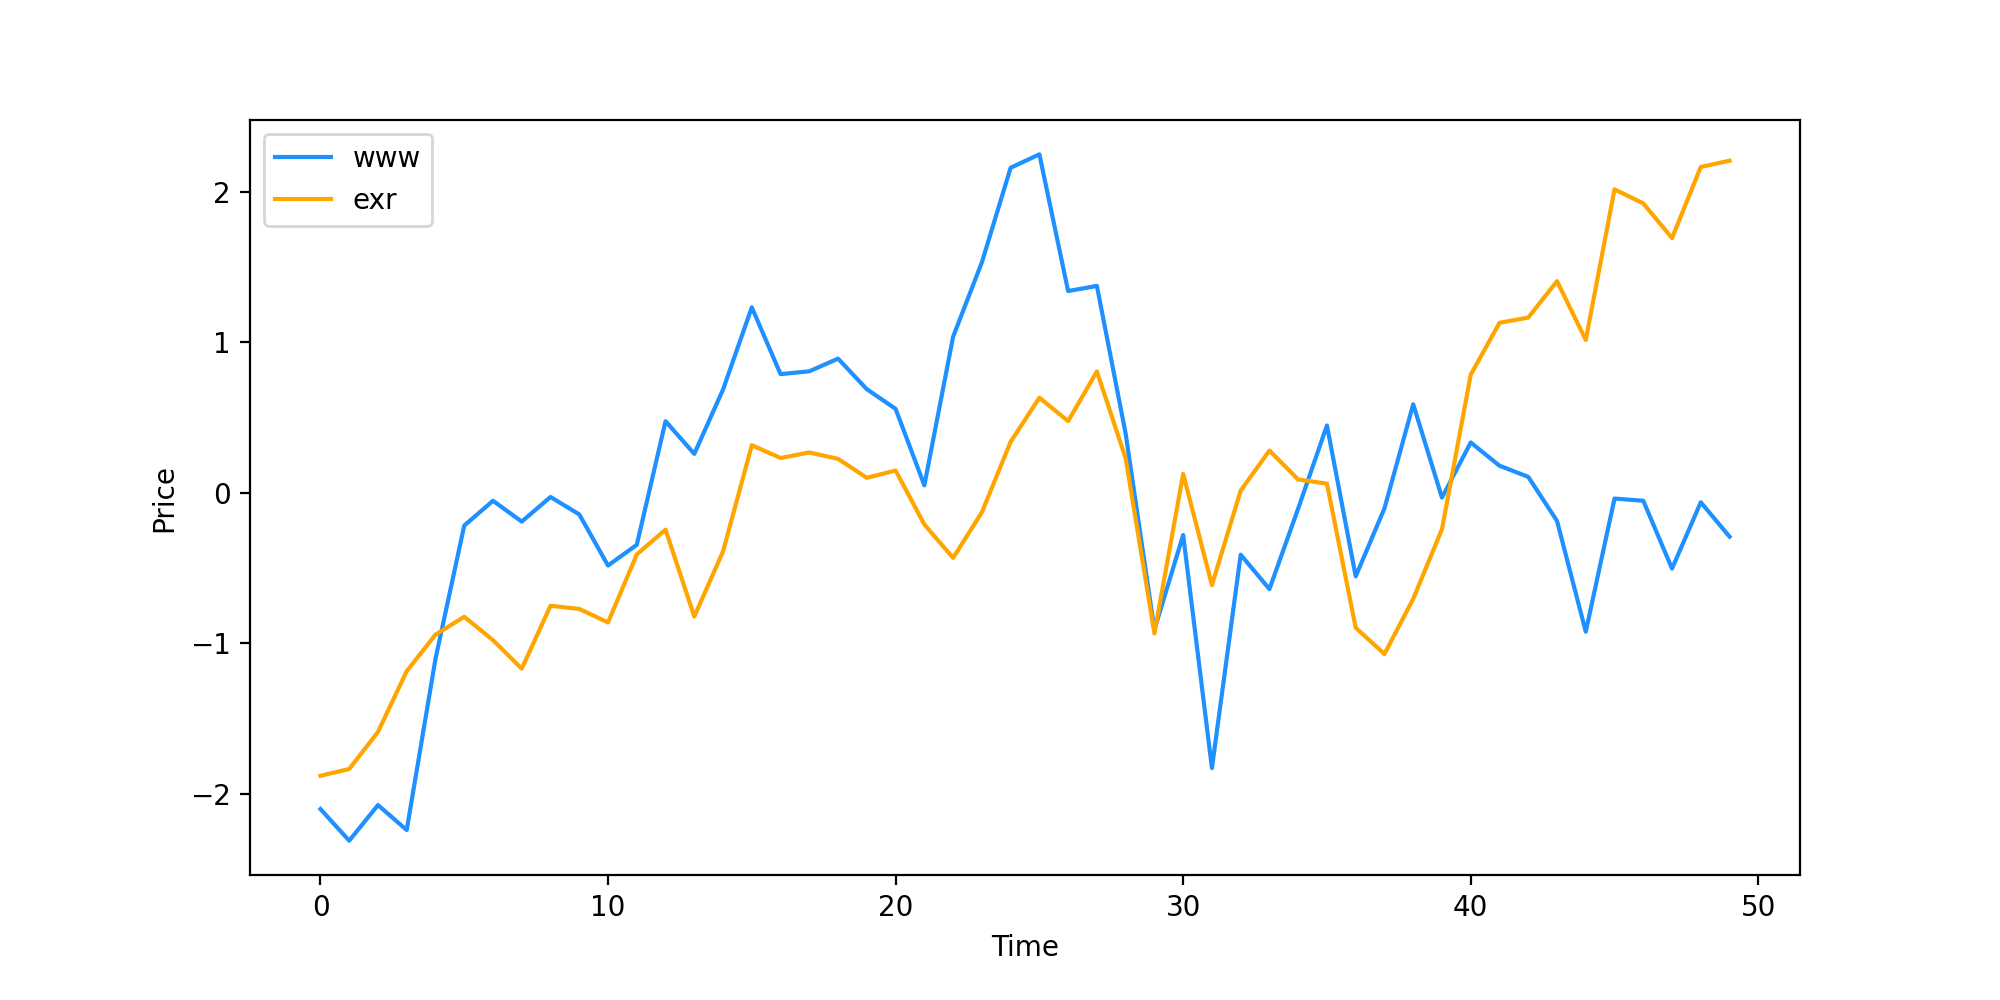
\includegraphics[width=0.4\columnwidth]{wwwexr1.png} 
    } 
    \subfigure[Path signature representation] { \label{fig:wwwexr2} 
    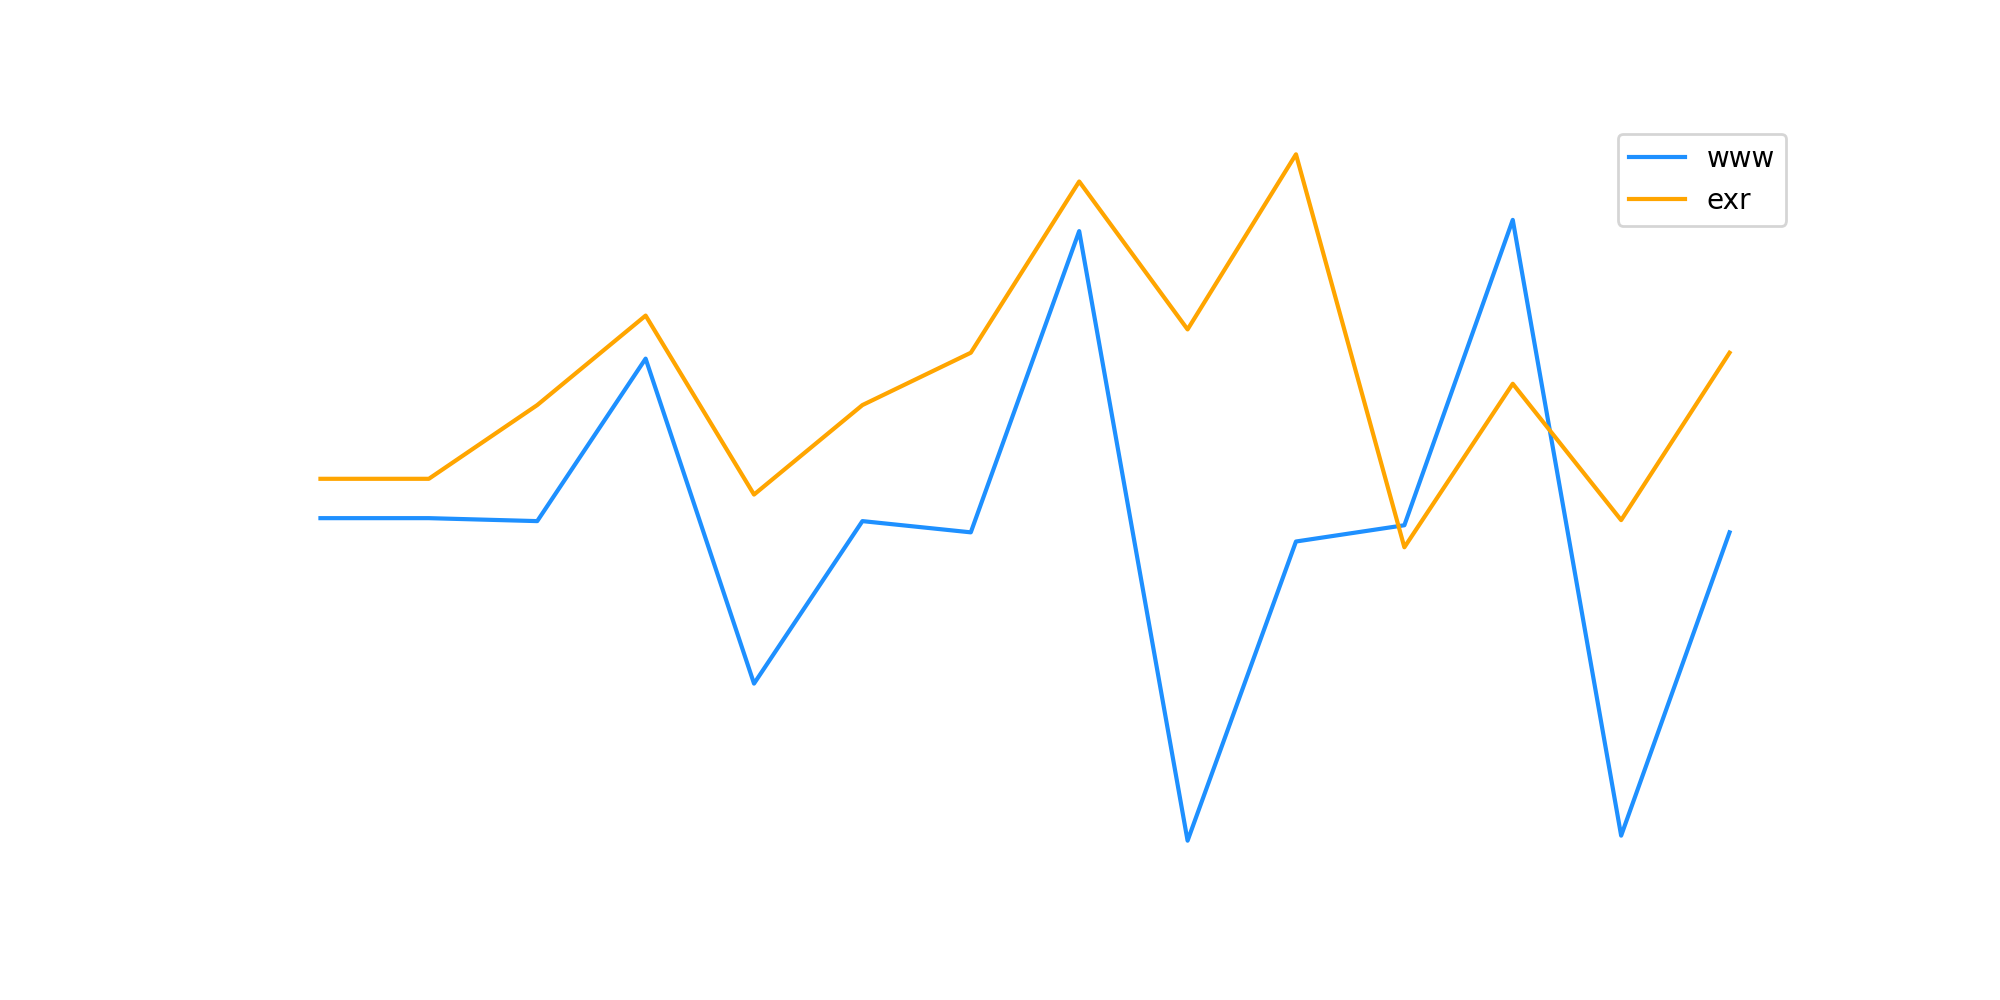
\includegraphics[width=0.4\columnwidth]{wwwexr2.png} 
    } 
    \caption{Example of path signature representation} 
    \label{fig:signature1} 
\end{figure} 


\section{Dynamic Feature Representations}
In contrast to static feature representation methods that produce identical results each execution, the middel block transforms sequences mainly by randomization and optimization. In this section, we introduce two major and novel dynamic feature representation methods for time-series data.
\subsection{Random convolutional kernels based sequence representation}
Convolutional neural networks are typically used in computer vision tasks, their success implicits that convolutional kernels may also be effective for extracting the features from time-series data, since in essence, time-series data have the same topology as images \cite{fawaz2020inceptiontime}. Different from transforming sequences with pre-defined patterns, convolutional neural networks can automatically detect patterns by learning. In addition, as stated by \cite{dempster2020rocket}, the learned kernels could also overlap with many types of features found in other methods, one supporting example is that they find that some of the learned kernels are similar to the extracted Shapelet patterns.\\
\\For a convolutional kernel, the most important parameters are its weights, and the process of updating weights can be treated as the extraction of features. Once the weights are determined, those kernels can be used to transform data. This process is done by using sliding dot product operation on the whole data, to produce a feature vector. For time-series data, a kernel is usually a 1-dimensional vector, after the convolution operation between the kernel and the input sequence, an additional bias term will be added. Apart from the two parameters weights and bias that are usually learned by updating, there are some user-defined parameters: (1) ``Size'' decides the length of the kernel; (2) ``Dilation'' decides the sampling gap of convolution operation; (3) ``Padding'' determinates whether appending values to the start and end the input sequence. These three parameters together decide the dimension of the produced vectors. \\
\\Typically, the weights updating process requires labelled data, hence convolutional kernel based methods are mainly used in classification tasks. However, researchers such as \cite{saxe2011random,pinto2009high} prove that random generated kernels can also be effective. This observation extends the use of convolutional kernels to unsupervised representation tasks. One possible way to make unsupervised kernels competitive with supervised kernels is increasing the number of random kernels. Due to the fact that those kernels' weights are not learned, their computation efficiency can be relatively high, which makes it possible to use a large number of kernels. One state-of-the-art time-series representation algorithm inheriting from such observation and idea is \textbf{ROCKET (RandOm Convolutional KErnel Transform)} \cite{dempster2020rocket}. It transforms time-series sequences by using a large set of kernels with random parameters (include all the 5 parameters mentioned above). The wide variety of kernels (especially kernels with different dilation and size) is said able to capturing patterns at different frequencies and scales. Similar to CNNs, ROCKET uses max pooling to sample features, besides, it uses an additional indexe - the proportion of positive values, to show whether a given pattern can be found within a time-series. For ROCKET, there is merely one user-defined parameter: the number of kernels $k$. Figure~\ref{fig:kernels1} shows an example of random kernels generated by ROCKET. \\
\begin{figure}[!htbp]
    \centering
    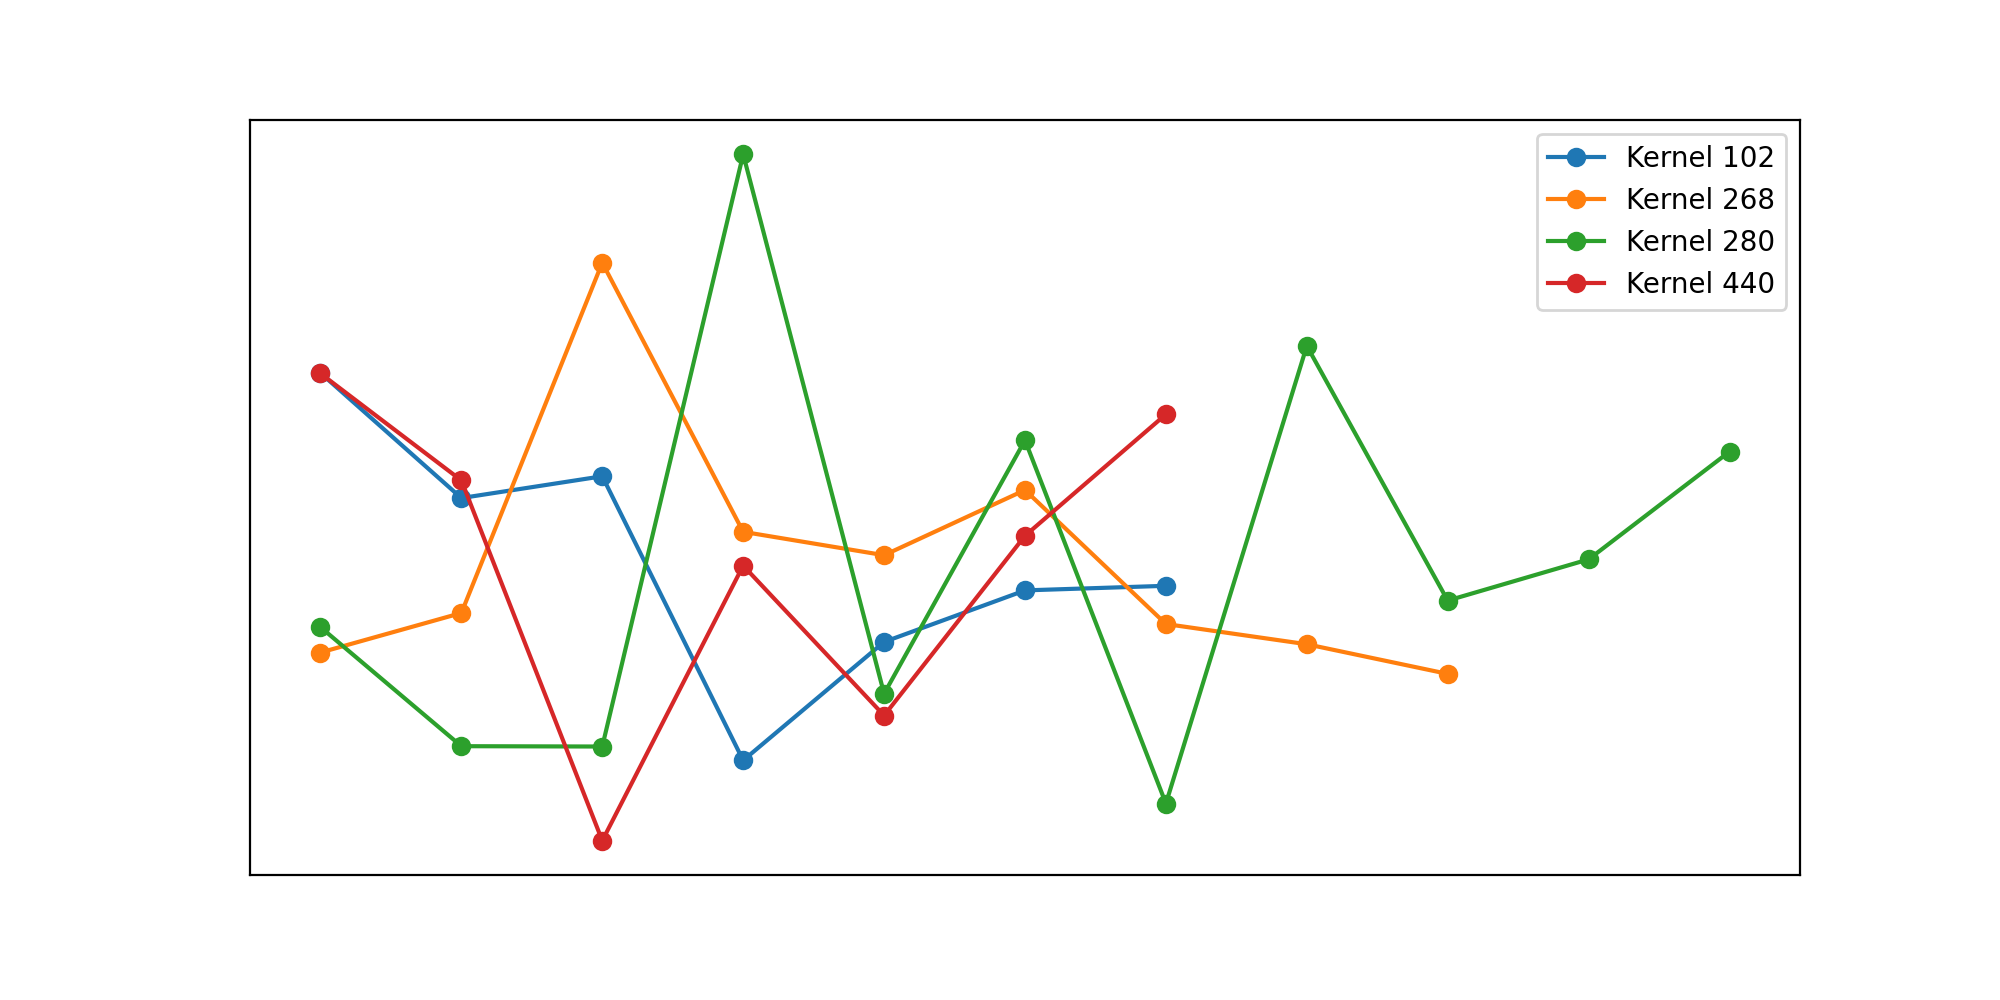
\includegraphics[width=0.6\columnwidth]{kernels1.png}
    \caption{Example of random convolutional kernels}
    \label{fig:kernels1}
\end{figure} 
\\Once the random kernels are generated, they can be used to transform the original sequences by convolution operation. Given a 1-d kernel $\omega$ with dilation $d$ and size $m$, and a sequence $X = (x_{1},\cdots, x_{T}) \in \mathbb{R}^{T} $, the convolution operation from $x_i$ is defined as:
\begin{equation}
    x_i * \omega = \sum_{j=0}^{m-1} x_{i+(j\times d)} \times \omega_j
\end{equation}
Each transformed feature map is then aggregated into two real value features: (1) the maximum value of it; (2) the proportion of positive value of it. And the final dimension of the transformed sequence is $2k$. One sample result of applying ROCKET to the records of ``NCS'' and ``GRVY'' in 2011 can be seen in Figure~\ref{fig:rocket1}. 
\begin{figure}[!htbp]
    \centering 
    \subfigure[Original sequences] { \label{fig:ncsgrvy1} 
    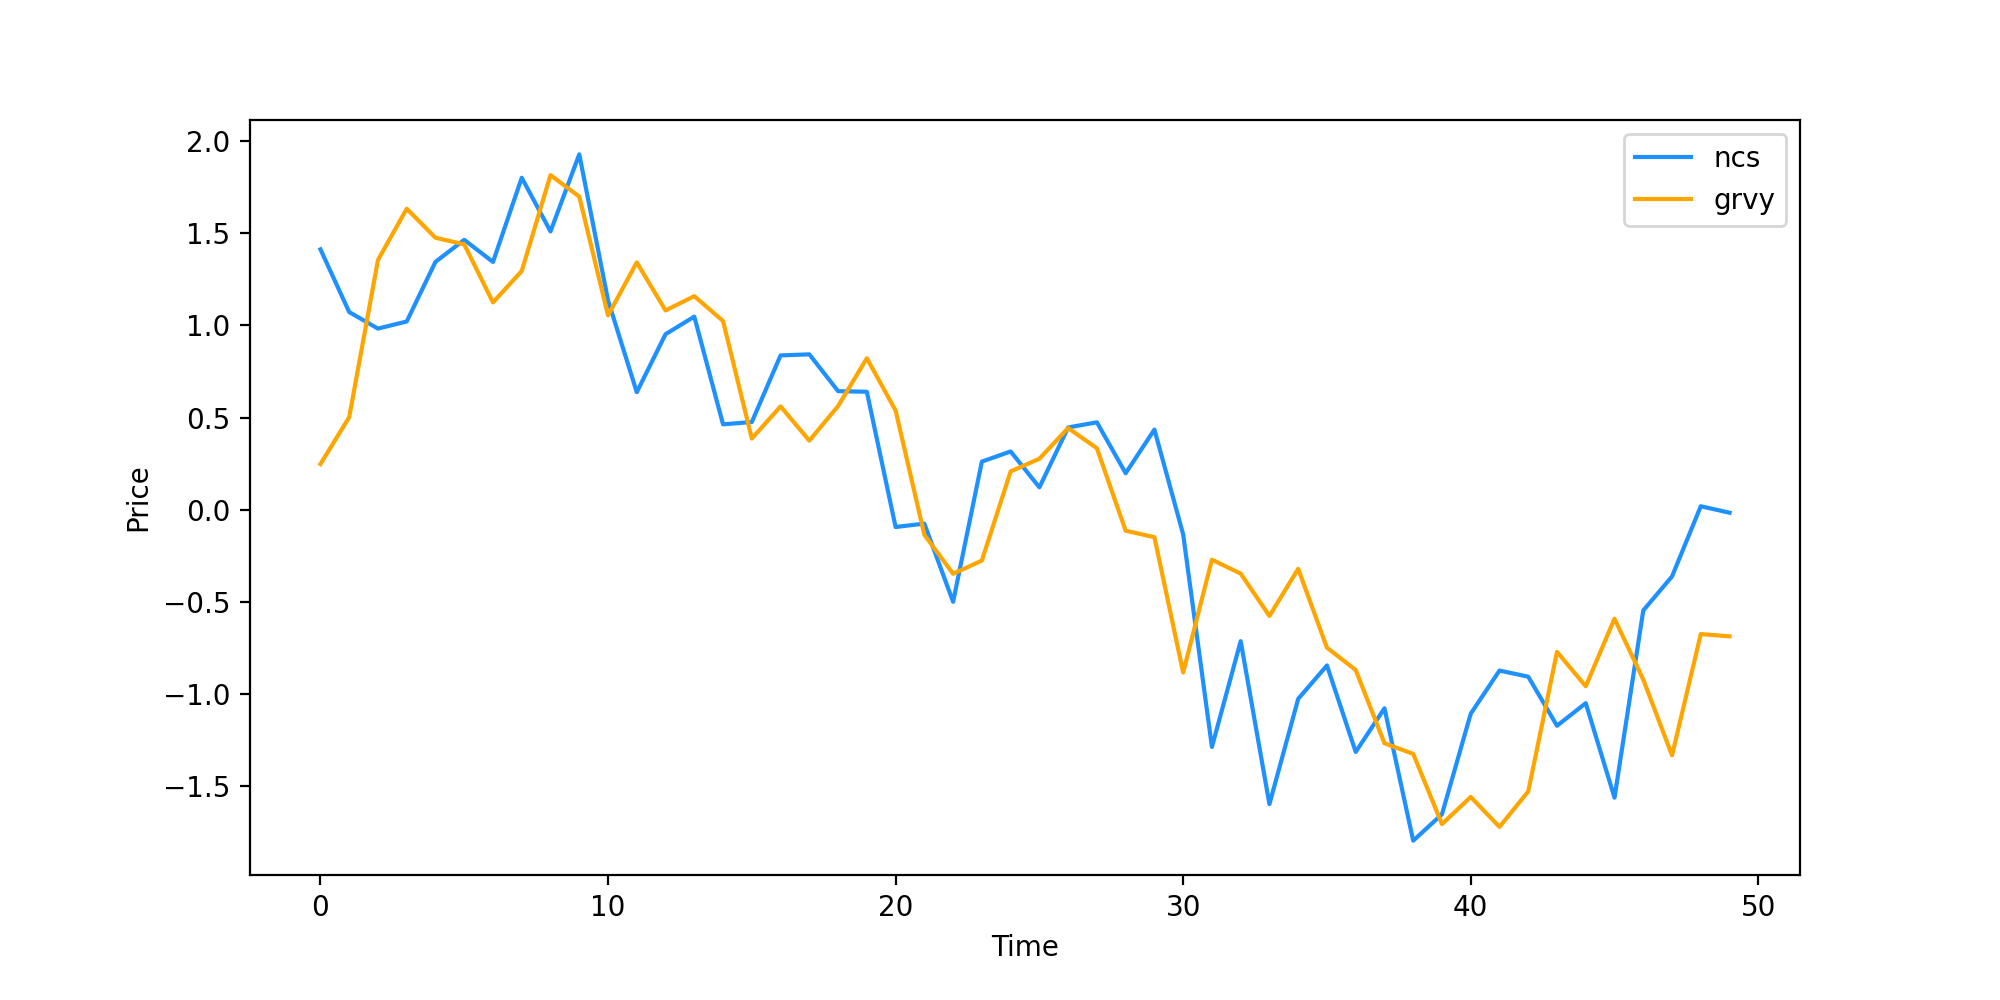
\includegraphics[width=0.4\columnwidth]{ncsgrvy1.png} 
    } 
    \subfigure[ROCKET representation] { \label{fig:ncsgrvy2} 
    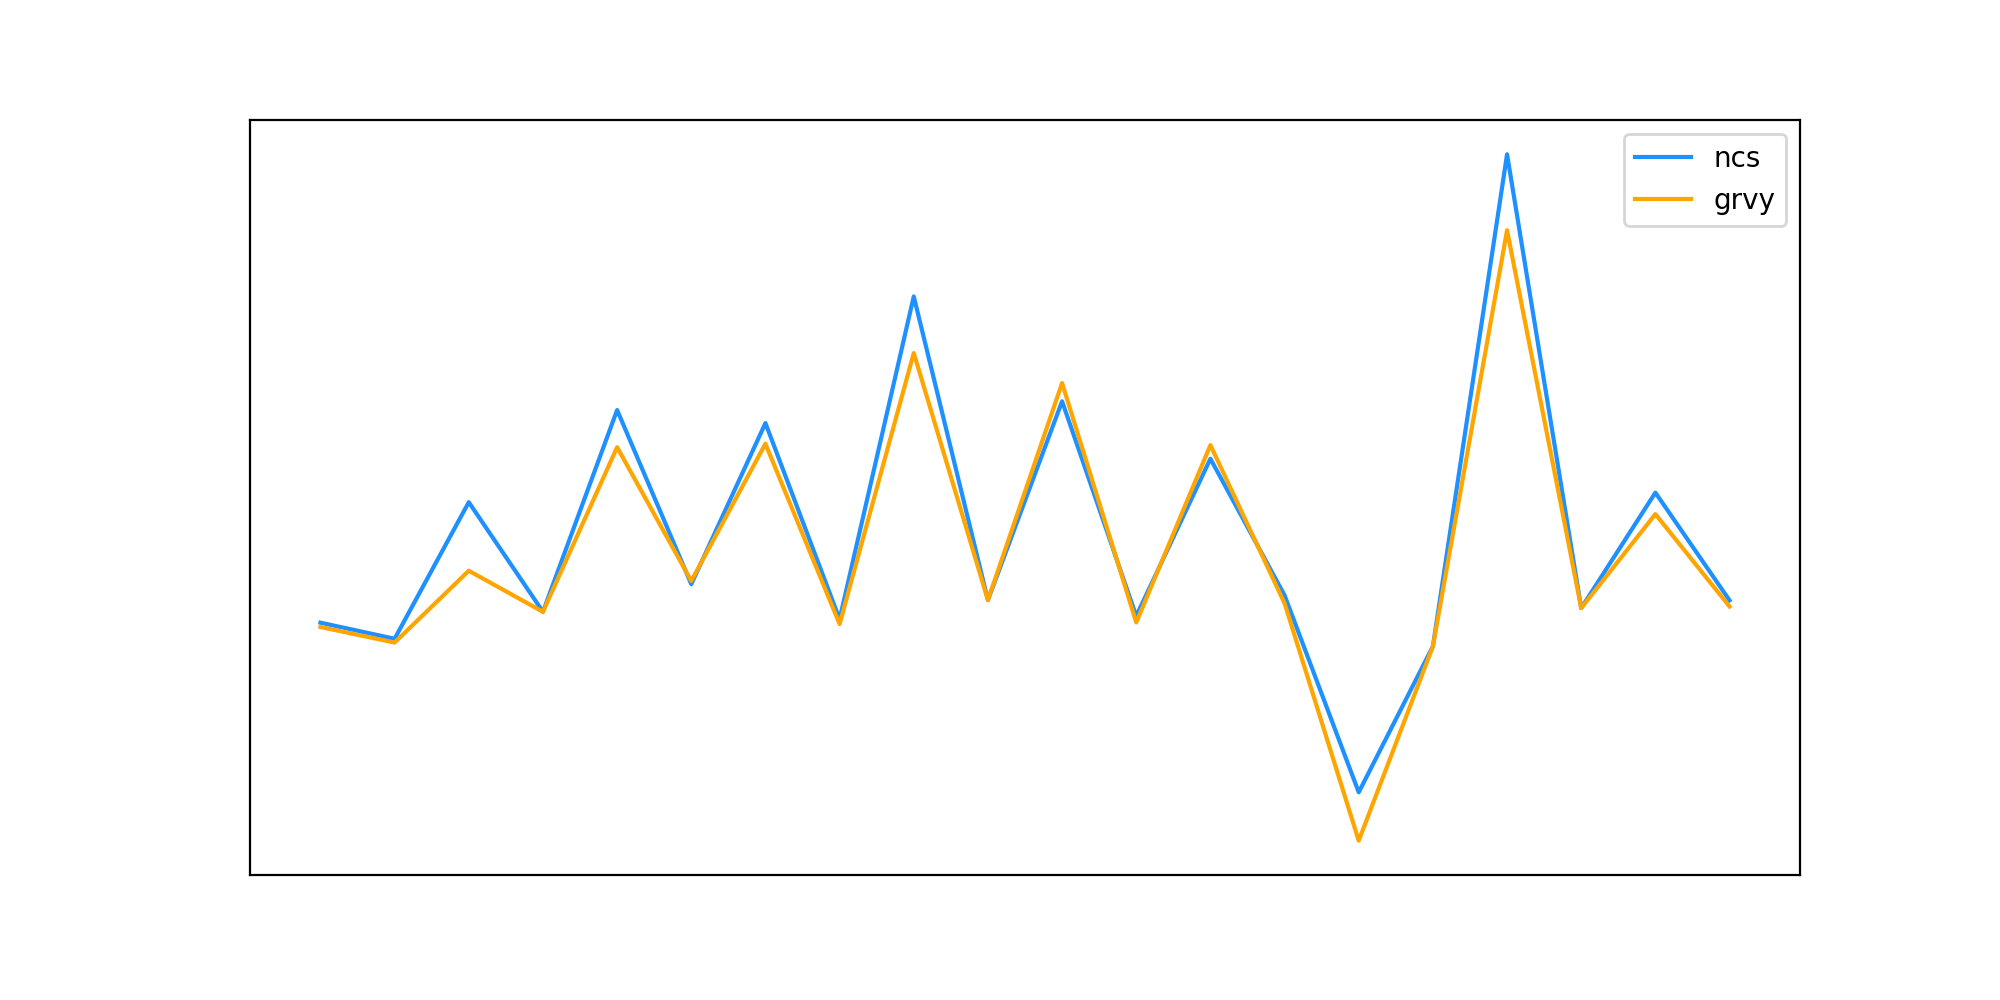
\includegraphics[width=0.4\columnwidth]{ncsgrvy2.png} 
    } 
    \caption{Example of ROCKET representation} 
    \label{fig:rocket1} 
\end{figure} 

\subsection{Self-supervised time-series representation learning}
Autoencoders are the core of various unsupervised learning tasks, they aim to extract the hidden structure of the input data, and transform the data into another representation with the least possible amount of distortion \cite{baldi2012autoencoders}. A typical autoencoder has two components: (1) an encoder that transform the original data into a new feature sapce; (2) an decoder that transforms the encoded sequences into output vectors. The traditional objective of an autoencoder is to minimize the difference of the output data and input data, and this is called reconstruction loss. Researchers such as \cite{malhotra2017timenet} and \cite{bianchi2019learning} adpot this scheme to transform time-series data, except that they use more sophisticated neural networks as the encoder and decoder. \\
\\Recently, due to the success of transformer architecture in unsupervised pre-training tasks, a relatively novel auto encoding objective \textbf{Masked Value Prediction (MVP)} is proposed by \cite{zerveas2020transformer}. This objective is analogue to Masked Language Modeling (MLM) of BERT, the main difference is that it is designed for time-series data. Literally, MVP works by setting some regions of the input sequence to 0 and ask the model to predict the masked values. Given an arbitrary sequence $X_m = (x_{m_1},\cdots, x_{m_T}) \in \mathbb{R}^{T \times D}$ as defined in Chapter~\ref{ch:Methodology}, MVP will produce an independent binary noise mask $M_m \in \mathbb{R}^{T \times D}$ for it. The mask has the same size with the input sequence, and the masking process is done by elementwise multiplication. A proportion $r$ is set to control the number of element (data point including all its features) to be maksed. It is worth noting that the authors do not simply use a Bernoulli distribution with parameter r to randomly mask the whole sequence, since such approaches could not guaranteed masked subsequences are long enough. They state that very short masked sequences can decrease the robustness of the model. Therefore, instead of using a Bernoulli distribution, they choose the state transition probabilities to decide the elements to be maksed. The length of each maksed segment is sampled from a geometric distribution with mean $l_m$, and each masked segment is succeeded by an unmasked segment of mean length $l_u=\frac{1-r}{r} l_m$ \cite{zerveas2020transformer}. With MVP, the head or the output layer can be a simple linear layer with parameters $W_o \in \mathbb{R}^{T \times N}$, $b_o \in \mathbb{R}^{N} $, where N is the dimension of the final sequence representation (the output of the last layer) $z_t \in \mathbb{R}^{N}$. For any sequence $X$, the model will output its estimate $X^\prime$. However, merely the prediction on the maksed regions will be used to compute the Mean Squared Error loss. Let $M = \{ (t,i): m_{t,i} = 0\}$ denotes the set of marked data points, the equation of MVP objective can be seen as follows:
\begin{equation} 
    X^\prime = W_o z_t + b_o 
\end{equation}
\begin{equation} 
    \mathcal{L}_{MSE} = \frac{1}{|M|} \sum_{t,i \in M} \sum (X\prime_{t,i} - X_{t,i}) ^ 2
\end{equation}
After the training, each sequence can be represented by its corresponding $z_t$. Theoretically, MVP can be applied to almost all neural networks. For better comparison, we choose the Time Series Transformer (TST) that used by the authors as the backbone. 
\begin{figure}[!htbp]
    \centering 
    \subfigure[Original sequences] { \label{fig:gpkwtisub1} 
    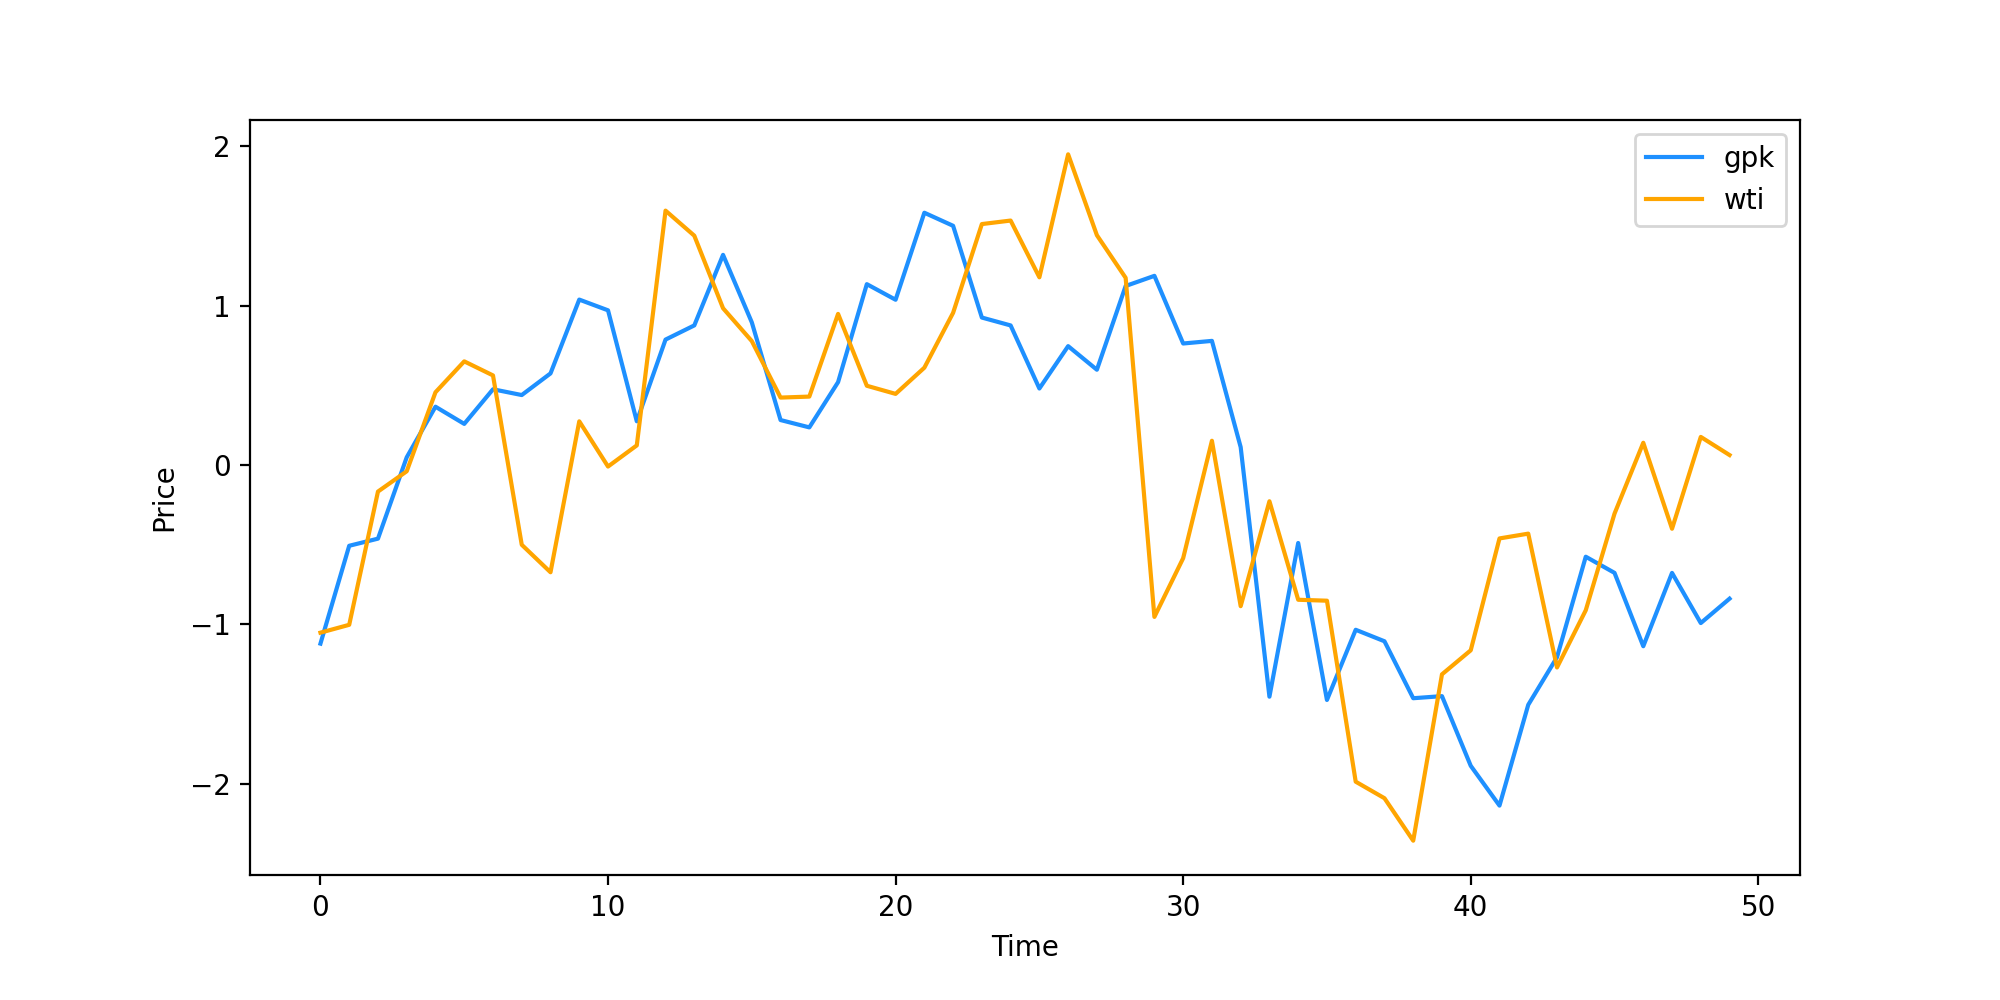
\includegraphics[width=0.4\columnwidth]{gpkwti1.png} 
    } 
    \subfigure[TST transformation] { \label{fig:gpkwtisub2} 
    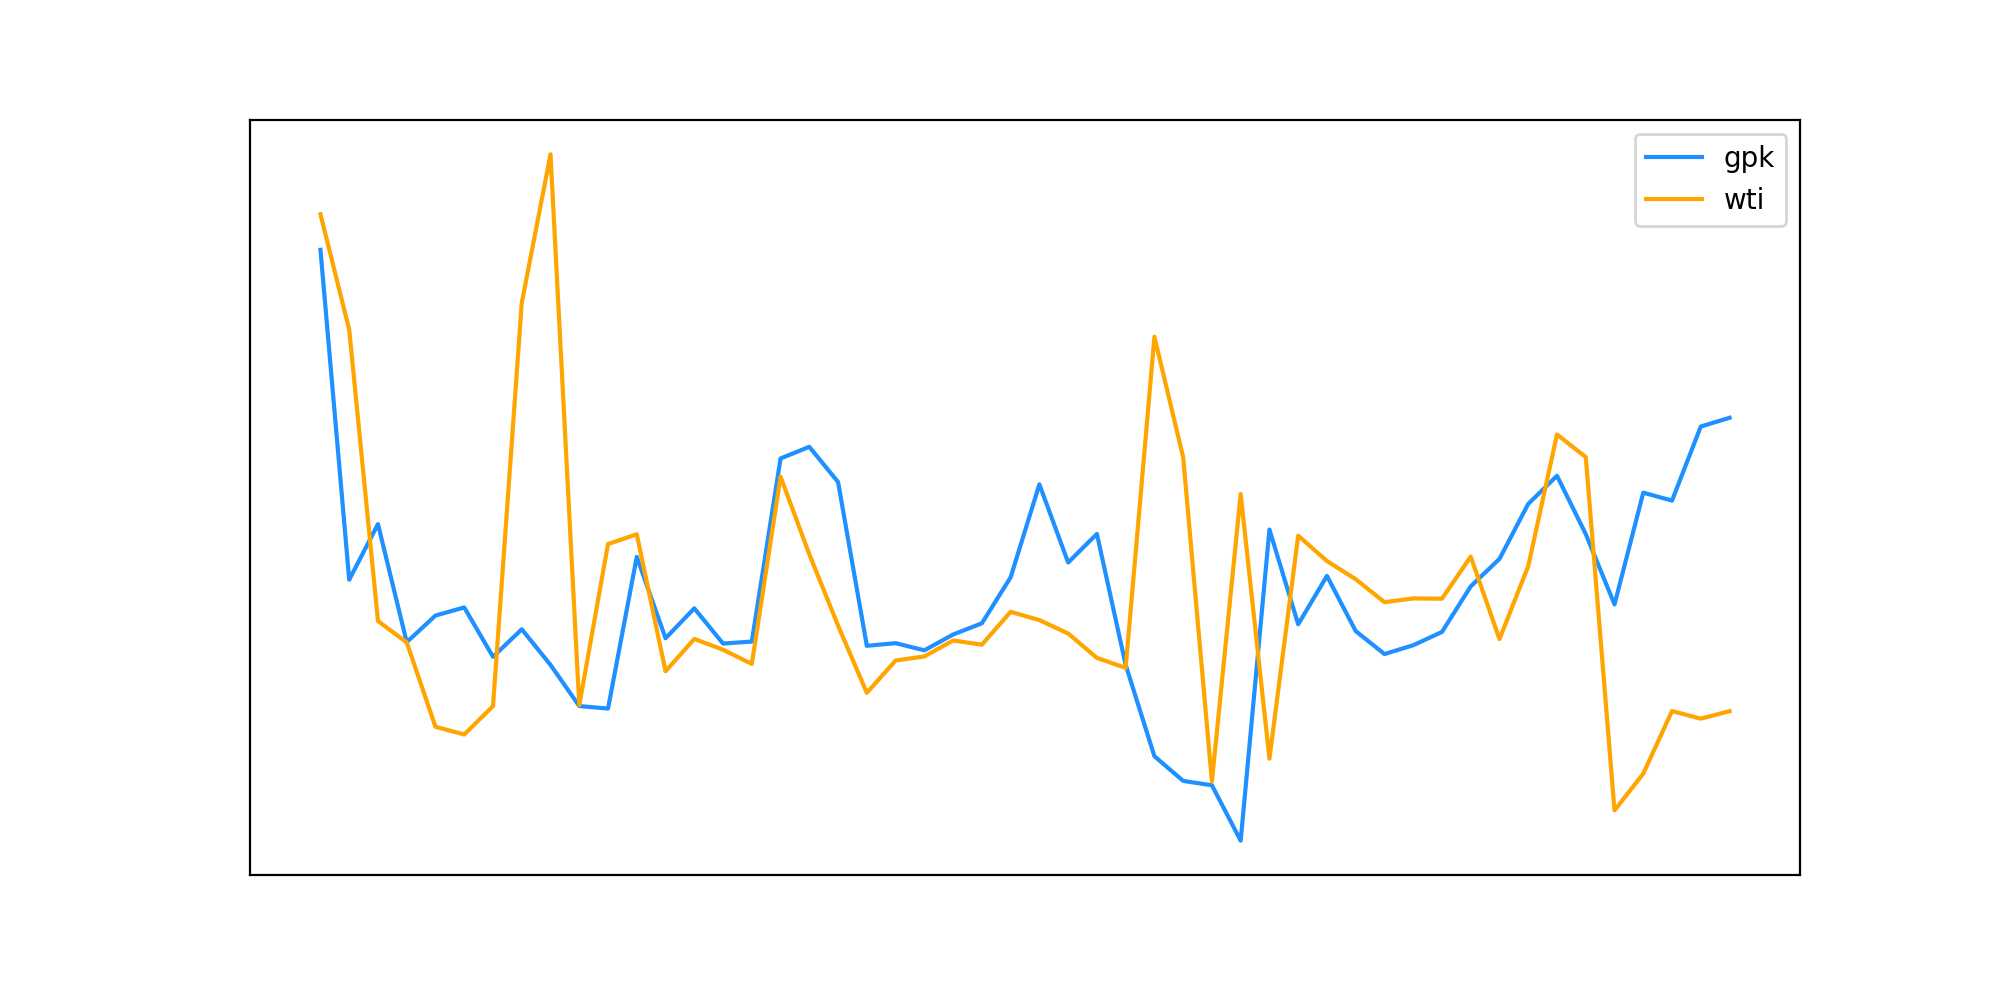
\includegraphics[width=0.4\columnwidth]{gpkwti2.png} 
    } 
    \caption{Example of self-supervised representation learning} 
    \label{fig:gpkwti1} 
\end{figure} 
Figure~\ref{fig:gpkwti1} shows an example of this transformation. The samples used here are the processed records of stock ``GPK'' and ``WTI'' in 2011. The relationship (both global and local) of the new representations is roughly comply with the original representations, except that the weights of different regions are uneven. 

\section{Shape-preserved representations}
\label{sec:pippaa}
All the representation algorithms introduced above transform the sequences into a new feature space and hence are hard to explain in visual. Therefore, we introduce another type of representation methods called shape-reversed representation. Such methods are usually compression-based, they are built on the observation that human can recognize a sequence even if that sequence are truncated or shortened. Note that compression-based methods are indeed can be categorized into Statistical Feature Representation, we add an independent section here because of their specialness. In Section~\ref{sec:compression1} we briefly introduce the three main sequence reduction algorithms. The first and simplest approach is resampling, which alters the frequency of the original data by interpolation. There are two types of resampling: upsampling and downsampling. The former one will increase the length of samples while the latter one will decrease the frequency of samples. Here we experiment with the \textbf{linear downsampling} approach, which simply choose $n$ data points with a fixed step from the original data. This transformation doesn't consider the structure of the original sequence and hence could lose some important information, but due to its simpleness, it is wildly used in many applications such as large sequence data storing. Note that the linear downsampling approach will not alter the original value. \\
\\One more advanced approach is Perceptually \textbf{Important Points (PIP) based sampling}. PIP based approaches are developed on the observation that human can recognize a sequence even when merely a small set of points of that sequence are given. \cite{zaib2004pattern} stated that the process of identifying PIPs is similar to the process of human cognition, where the general shpae of the data will be first recognized and the the details. In the context of data mining, PIPs are mainly used for dimension compression or sequence segmentation. The general process of this algorithm is introduced in Section~\ref{sec:compression1}, here we mainly present the equations to find salient points. In PIP identification process, three distance metrics are used: the Euclidean distance $d_E$, the perpendicular distance $d_P$ and the vertical distance $d_V$. In a simple example, let $X = \{x_1,x_2, \cdots, x_l\}$ denotes a 1-d sequence of length $l$, $x_t = (t, x_t)$ and $ x_{t+T} = (t+T,x_{t+T})$ denote two adjacent PIPs. The Euclidean distance $d_E$ of an intermediate point $x_i = (i, x_i)$, $t < i < t+T$, is defined in Equation \ref{eq:euclideandoulbe}. 
\begin{equation}
    \label{eq:euclideandoulbe}
    d_E(x_i, x_t, x_{t+T}) = d_E(x_i, x_t) + d_E(x_i, x_{t+T})
\end{equation}
The vertical distance and perpendicular distance are computed from the line across the two PIPs. Assuming that $(i,z_i)$ is a point on that line, $z_i = si+c$, the slope of that line is $s = \frac{x_{t+T} - x_t}{T}$ and the constant term is $c = x_t - st$, the perpendicular distance $d_P$ and the vertical distance $d_V$ between the intermediate points and the two PIPs are defined in Equation \ref{eq:perpendicular} and \ref{eq:vertical} respectively. The next PIP is select as the intermediate point $x_i^* = (i^*, x_{i^*})$ that maximizes the three distances. The equation can be seen in Equation \ref{eq:pipselect}.
\begin{equation}
    \label{eq:perpendicular}
    d_P(x_i, x_t, x_{t+T}) = \frac{|si+c-x_i|}{\sqrt{s^2+1}}
\end{equation}
\begin{equation}
    \label{eq:vertical}
    d_V(x_i, x_t, x_{t+T}) = |si+c-x_i|
\end{equation}
\begin{equation}
    \label{eq:pipselect}
    i^* = arg\max_i(d(x_i, x_t, x_{t+T}))
\end{equation}
According to \cite{zaib2004pattern}, PIP-based compression approaches could alleviate the effect of missing data as long as the main points to form the sequence exist. This property can help to reach global scaling invariance and occlusion invariance. The main drawback of this approach is that the distribution of salient points could be uneven, which may change the shape of certain sequences. Note that similar to linear downsampling, this approach will not change the original value.\\
\\ The third compression approach is \textbf{Piecewise Aggregate Approximation (PAA)}. As introduced in Section~\ref{sec:compression1}, this approach will divide the data into $n$ equal-sized segments, and use a vector of mean values of segments to represent the original data. The compressed data can be represented as $P\prime = {p_1\prime, \cdots, p_n\prime}$, where the $i_{th}$ element of $P\prime$ can be calculated by Equation \ref{eq:paa1}, where N is the length of original sequence.
\begin{equation}
    \label{eq:paa1}
    p_i\prime = \frac{N}{n} \sum_{j=\frac{n}{N}(i-1)+1}^{\frac{n}{N}i} p_j
\end{equation}

\begin{figure}[!htbp]
    \centering 
    \subfigure[Closing price of IBA in 2011] { \label{fig:iba2} 
    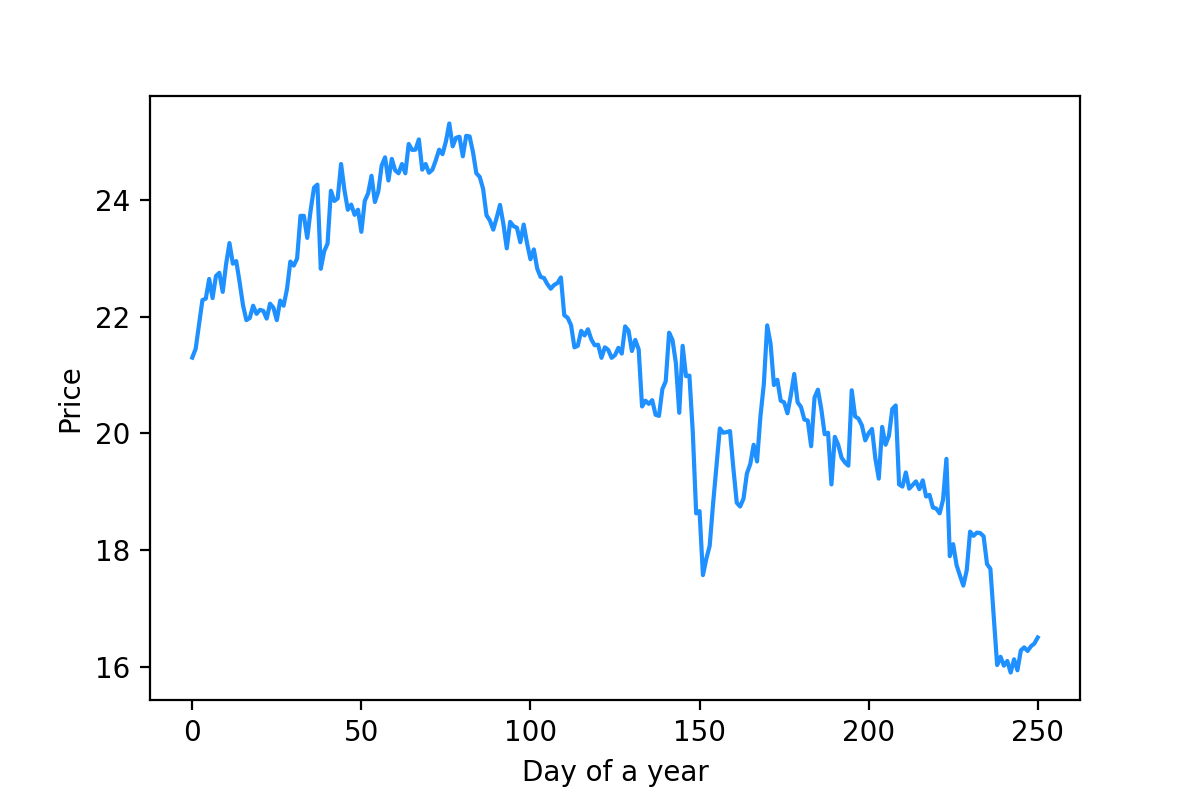
\includegraphics[width=0.45\columnwidth]{iba2.png} 
    } 
    \subfigure[Comparison of 3 approaches] { \label{fig:pippaacompare1} 
    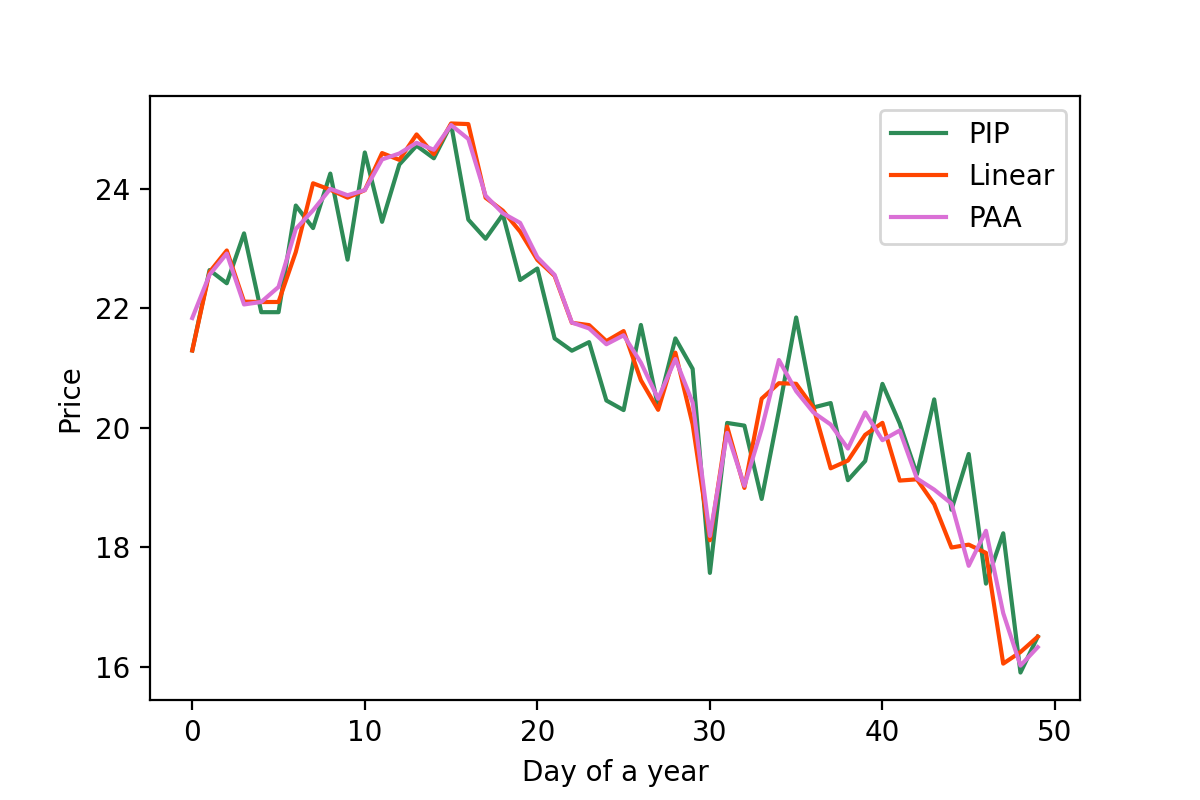
\includegraphics[width=0.45\columnwidth]{pippaacompare1.png} 
    } 
    \subfigure[Result of linear downsampling] { \label{fig:linear1} 
    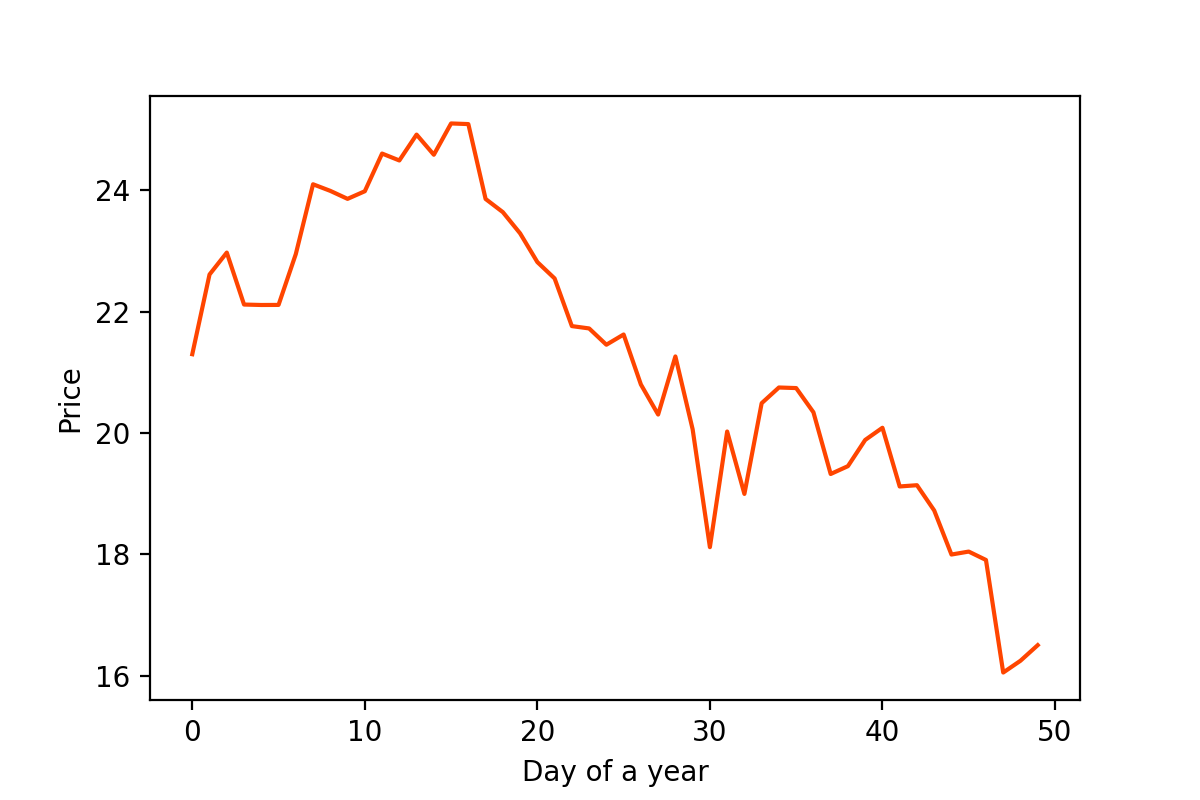
\includegraphics[width=0.3\columnwidth]{linear_sampling.png} 
    }
    \subfigure[Result of PIP] { \label{fig:pip2} 
    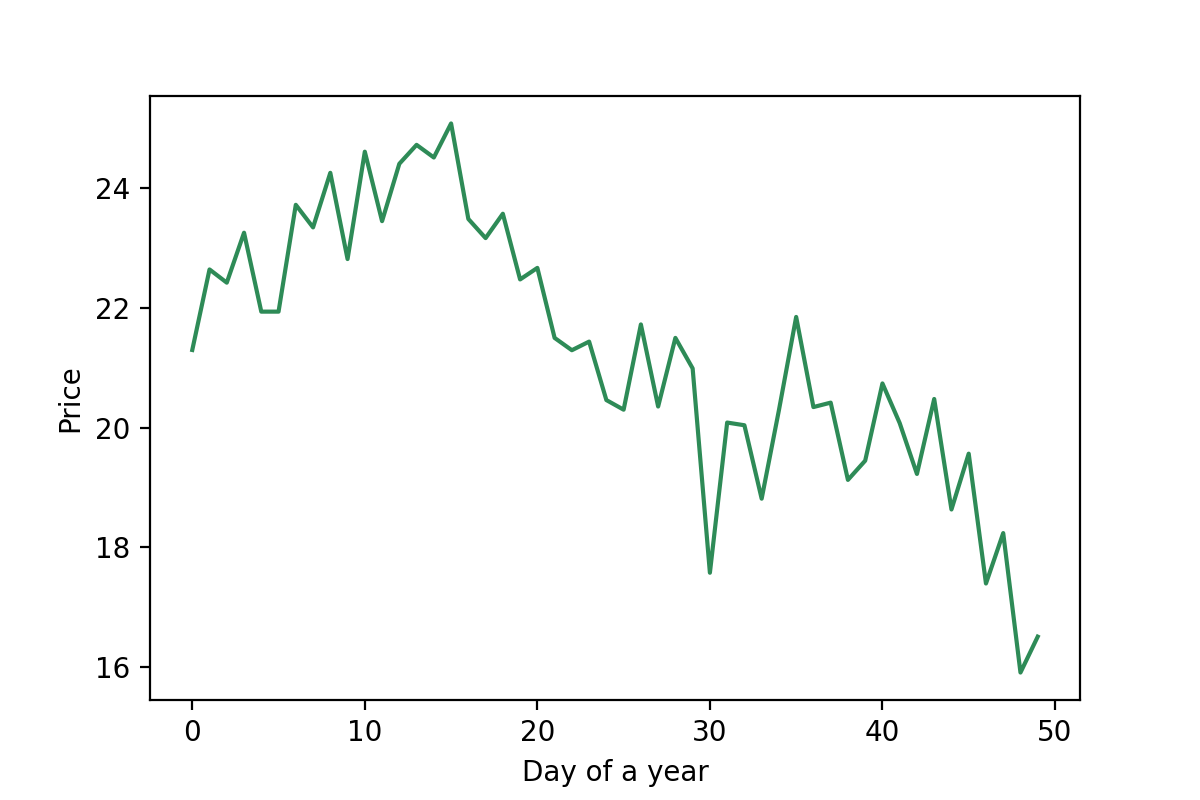
\includegraphics[width=0.3\columnwidth]{pip_iba_50.png} 
    } 
    \subfigure[Result of PAA] { \label{fig:paa2} 
    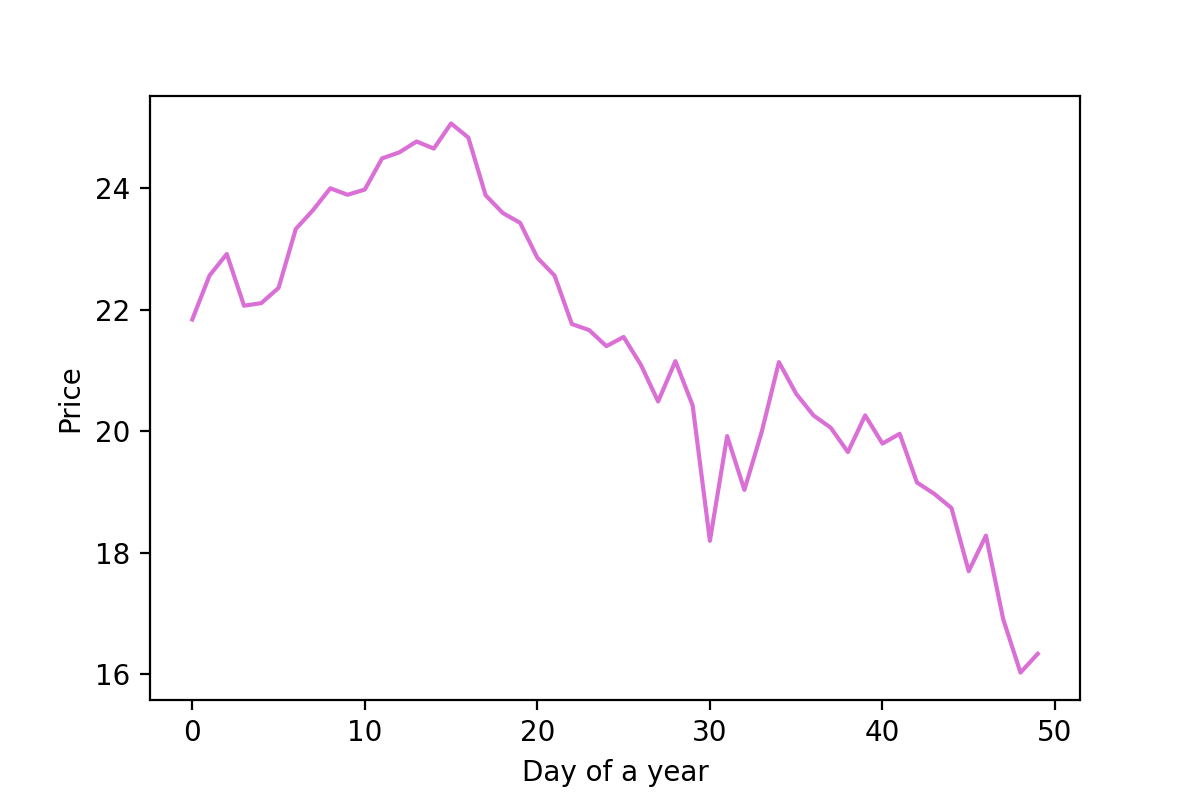
\includegraphics[width=0.3\columnwidth]{ppa_50.png} 
    } 
    \caption{ Compression results (n=50) } 
    \label{fig:compression2} 
\end{figure} 
Figure~\ref{fig:compression2} shows the results of using these approaches. Similarly, the sample used here is the un-modified closing price sequence of IBA in 2011 (Figure~\ref{fig:iba2}). The general comparison of the three approaches can be seen at the top right, where the green line represents the PIP-compressed sequence, orange line represents the linear-downsampled sequence and the purple line is the PAA-compressed sequence. The original sequence contains 251 data points while that of the compressed sequence is set to 50, the compression ratio $r=n/N$ is roughly 20\%. The figures in the second row are the results of the three approaches respectively. From the second row, we can find that all the three approaches can produce recognizable shapes of the original sequence. Although the global shapes of the three modified sequences are similar, the local shapes can vary - PIP reserves more fluctuations and turning points while the others does not.
As shown in the top right figure, linear downsampling and PAA based compression overlap at most regions, especially in the region between 0 and 30. Both of them smooth the region between 15 and 20 while PIP reserves some points of that region. As mentioned before, downsampling has no idea of which point is more important, hence it can miss some turning points, and this is proved in region 35 to 50. PAA can be treated as an mean filter in terms of denoising, and the drawbacks are discussed in Section~\ref{sec:denosing}. \\
\\To compare the three method objectively, we conduct experiments based on the similar between sequences. The results can be seen in Table~\ref{tab:compression1}. Same with the experiment conducted in Section~\ref{sec:denosing}, we randomly choose 20 similar stocks from our dataset as the samples, and use the mean values pair-wise distances as the metrics. One difference is that in this experiment, data are not normalised. The experimental results shows that there is no significant difference among the three approaches. One interesting observation is that the simplest downsampling method gets the highest markers on 3 indexes, especially on DWT, which we think is the most appropriate index under our guideline. 
\begin{table}[!htbp]
    \centering
    \hspace{0.5cm}
    \begin{tabular}{|c|c|c|c|c|}
        \hline
         & DWT & Cosine & Euclidean & Correlation \\ \hline
        Downsampling & 177.077 & 0.020 & 180.243 & 0.121 \\ \hline
        PIP & 185.685 & 0.020 & 189.590 & 0.193 \\ \hline
        PAA & 188.722 & 0.020 & 191.760 & 0.137 \\ \hline
    \end{tabular}
    \caption{Sequences compression results}
    \label{tab:compression1}
\end{table}
It's worth noting that the choosing of the sequence length ``c'' is a classical tradeoff between the fidelity and dimensionality. According to \cite{keogh2000scaling}, the ``best'' compression rate highly depends on the internal structure of the data and the application. The effect of different sequence length is examined in clustering results.